\documentclass[polish]{aghengthesis}

\usepackage[utf8]{inputenc}
\usepackage{url}
\usepackage{subfig}
\usepackage{float}
\usepackage{tabularx}
\usepackage{ragged2e}
\usepackage{booktabs}
\usepackage{multirow}
\usepackage{grffile}
\usepackage{indentfirst}
\usepackage{caption}
\usepackage{listings}
\usepackage[ruled,linesnumbered,lined]{algorithm2e}
\usepackage[bookmarks=false]{hyperref}
\usepackage{placeins}

\hypersetup{colorlinks,
  linkcolor=blue,
  citecolor=blue,
  urlcolor=blue}

\usepackage[svgnames]{xcolor}
\usepackage{inconsolata}

\usepackage{csquotes}
\DeclareQuoteStyle[quotes]{polish}
  {\quotedblbase}
  {\textquotedblright}
  [0.05em]
  {\quotesinglbase}
  {\fixligatures\textquoteright}
\DeclareQuoteAlias[quotes]{polish}{polish}

\usepackage[nottoc]{tocbibind}

\usepackage[
style=numeric,
% sorting=nyt,
sorting=none,
isbn=false,
doi=true,
url=true,
backref=false,
backrefstyle=none,
maxnames=10,
giveninits=true,
abbreviate=true,
defernumbers=false,
backend=biber]{biblatex}
\addbibresource{main.bib}


\lstdefinelanguage{JavaScript}{
  keywords={typeof, new, true, false, catch, await, function, return, null, undefined, void, catch, switch, var, if, in, while, do, else, case, break},
  ndkeywords={class, export, async, boolean, throw, implements, import, this},
  % identifierstyle=\color{black},
  sensitive=false,
  comment=[l]{//},
  morecomment=[s]{/*}{*/},
  morestring=[b]',
  morestring=[b]"
}

\lstset{
  language=JavaScript,
  backgroundcolor=\color{gray!5},
  commentstyle=\it\color{Green},
  keywordstyle=\color{Red},
  ndkeywordstyle=\color{Red},
  stringstyle=\color{Blue},
  numberstyle=\tiny\color{Black}, 
  extendedchars=true,
  basicstyle=\footnotesize\ttfamily,
  % frame=single, %shadowbox, 
  rulecolor=\color{black!30},
  title=\lstname,
  breaklines=true,
  breakatwhitespace=true,
  framextopmargin=2pt,
  framexbottommargin=2pt,
  showstringspaces=false,
  showspaces=false,
  numbers=left,
  numberstyle=\footnotesize,
  numbersep=5pt,
  tabsize=2,
  breaklines=true,
  showtabs=false,        
  showstringspaces=false,
  captionpos=b,
  escapeinside=`',
  literate={`}{\textasciigrave}1,
  mathescape=true,
}

\newcommand{\dollar}{\mbox{\textdollar}}


\SetAlgorithmName{\LangAlgorithm}{\LangAlgorithmRef}{\LangListOfAlgorithms}
\newcommand{\listofalgorithmes}{\tocfile{\listalgorithmcfname}{loa}}

\renewcommand{\lstlistingname}{\LangListing}
\renewcommand\lstlistlistingname{\LangListOfListings}

\renewcommand{\lstlistoflistings}{\begingroup
\tocfile{\lstlistlistingname}{lol}
\endgroup}

% Definicje nowych rodzajów kolumn w tabeli
\newcolumntype{Y}{>{\small\centering\arraybackslash}X}
%\newcolumntype{b}{>{\hsize=1.6\hsize}Y}
%\newcolumntype{m}{>{\hsize=.6\hsize}Y}
%\newcolumntype{s}{>{\hsize=.4\hsize}Y}

\captionsetup[figure]{skip=5pt,position=bottom}
\captionsetup[table]{skip=5pt,position=top}

%%%%%%%%%%%%%%%%%%%%%%%%%%%%%%%%%%%%%%%%%%%%%%%%%%%%%%%%%%%%%%%%%%%%%%%%%%%%%%%

\author{Szymon Idec, Jakub Karbowski, Karol Śliwa}

\titlePL{Wirtualny asystent gry w brydża}
\titleEN{A virtual bridge game assistant}

\fieldofstudy{Informatyka}

%\typeofstudies{Stacjonarne}

\supervisor{dr hab. inż.\ Maciej Woźniak}

\date{\the\year}

%%%%%%%%%%%%%%%%%%%%%%%%%%%%%%%%%%%%%%%%%%%%%%%%%%%%%%%%%%%%%%%%%%%%%%%%%%%%%%%

\begin{document}

\maketitle

\tableofcontents

%%%%%%%%%%%%%%%%%%%%%%%%%%%%%%%%%%%%%%%%%%%%%%%%%%%%%%%%%%%%%%%%%%%%%%%%%%%%%%%

\chapter{\ChapterTitleProjectVision}
\label{sec:cel-wizja}

%%%

\section{Charakterystyka problemu}

Gry karciane, takie jak brydż, cieszą się dużą popularnością na całym świecie.
Jednakże wiele osób ma trudności w~znalezieniu odpowiednich partnerów do gry,
szczególnie w przypadku osób początkujących, które nie posiadają jeszcze
szerokiego kręgu znajomych zainteresowanych tą grą. W~takiej sytuacji, osoby
chcące nauczyć się gry w~brydża lub doskonalić swoje umiejętności, często
zniechęcają się do dalszego uczestnictwa w~rozgrywkach.

Ponadto, brydż jest grą wymagającą nie tylko umiejętności logicznego myślenia
i~strategii, ale także zdolności do skutecznej komunikacji i~współpracy
z~partnerem. Wielu początkujących graczy nie jest w~stanie zagrać pełnej
i~satysfakcjonującej gry, gdyż nie posiadają odpowiedniego doświadczenia
i~umiejętności. Dodatkowo niektórzy mogą nie być w stanie znaleźć
odpowiedniego partnera posiadającego podobny styl gry lub
rozumiejącego stosowaną strategię.

W~związku z~powyższymi problemami zidentyfikowano potrzebę opracowania
aplikacji do gry w brydża, która umożliwiłaby grę z~wirtualnym asystentem
na poziomie umiejętności dostosowanym do użytkownika, zapewniającym satysfakcjonującą
rozgrywkę oraz możliwość nauki i~doskonalenia umiejętności gry w~brydża.

%%%

\section{Motywacja projektu}

\begin{figure}
    \centering
    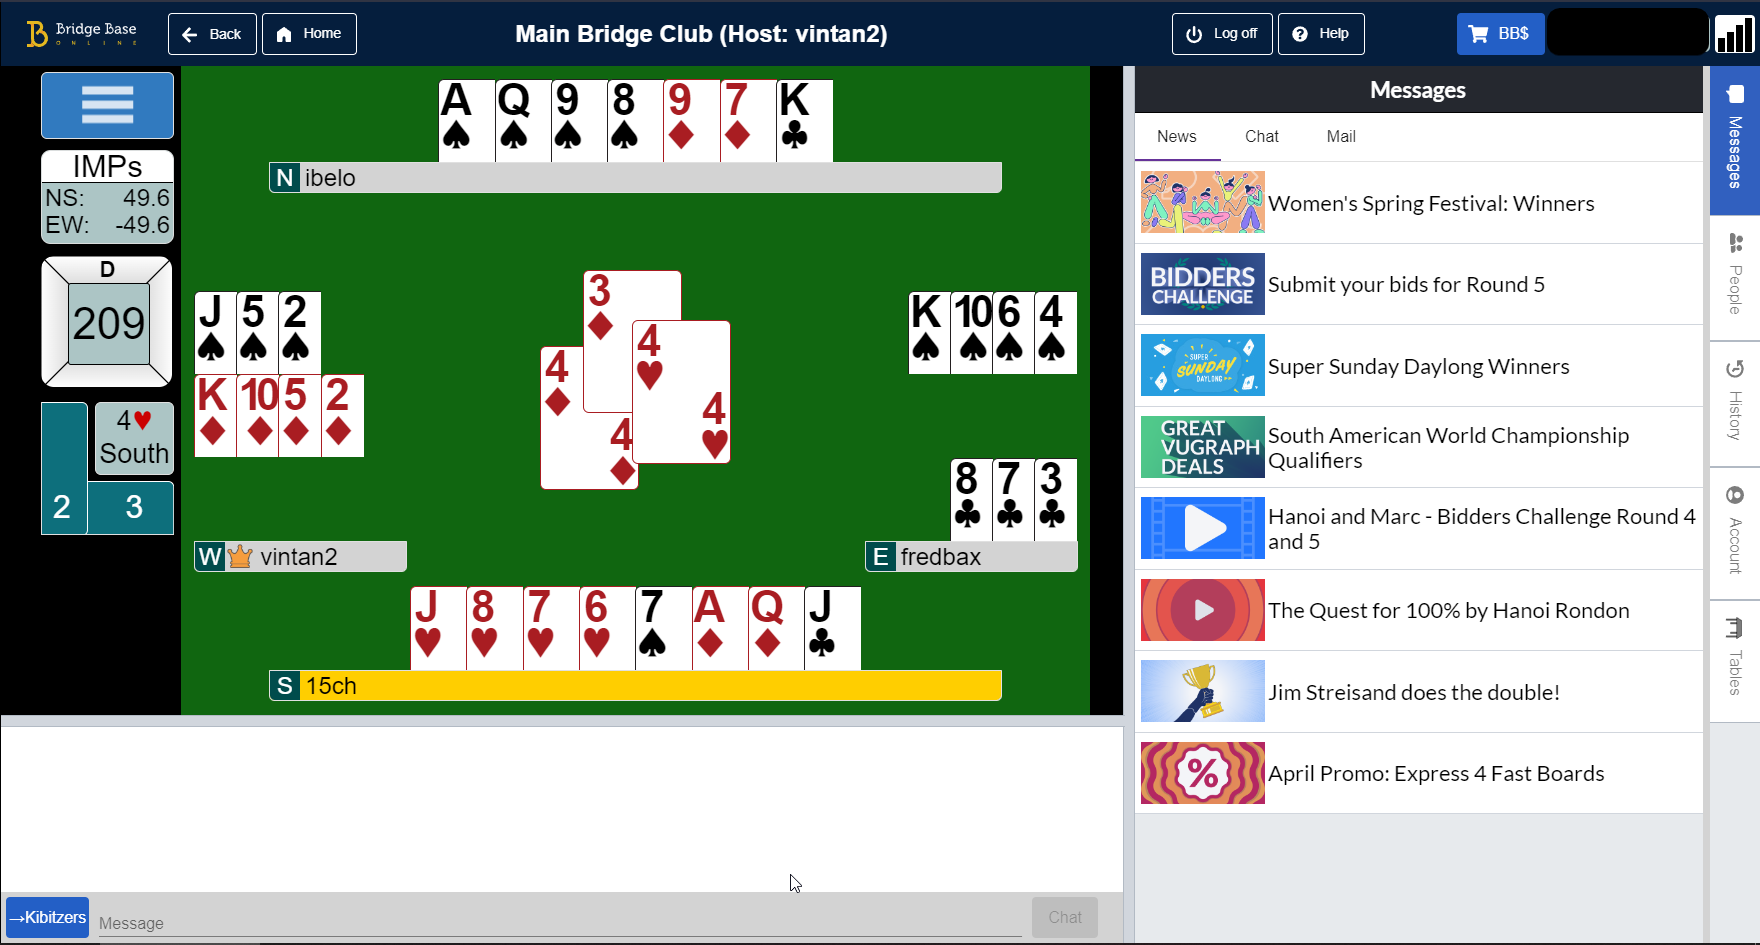
\includegraphics[width=0.9\textwidth]{img/brydz-platformy/bridgebase.png}
    \caption{Rozgrywka brydża na platformie Bridge Base}
    \label{fig:bridge-base}
\end{figure}

\begin{figure}
    \centering
    \subfloat[Główny ekran rozgrywki]{
        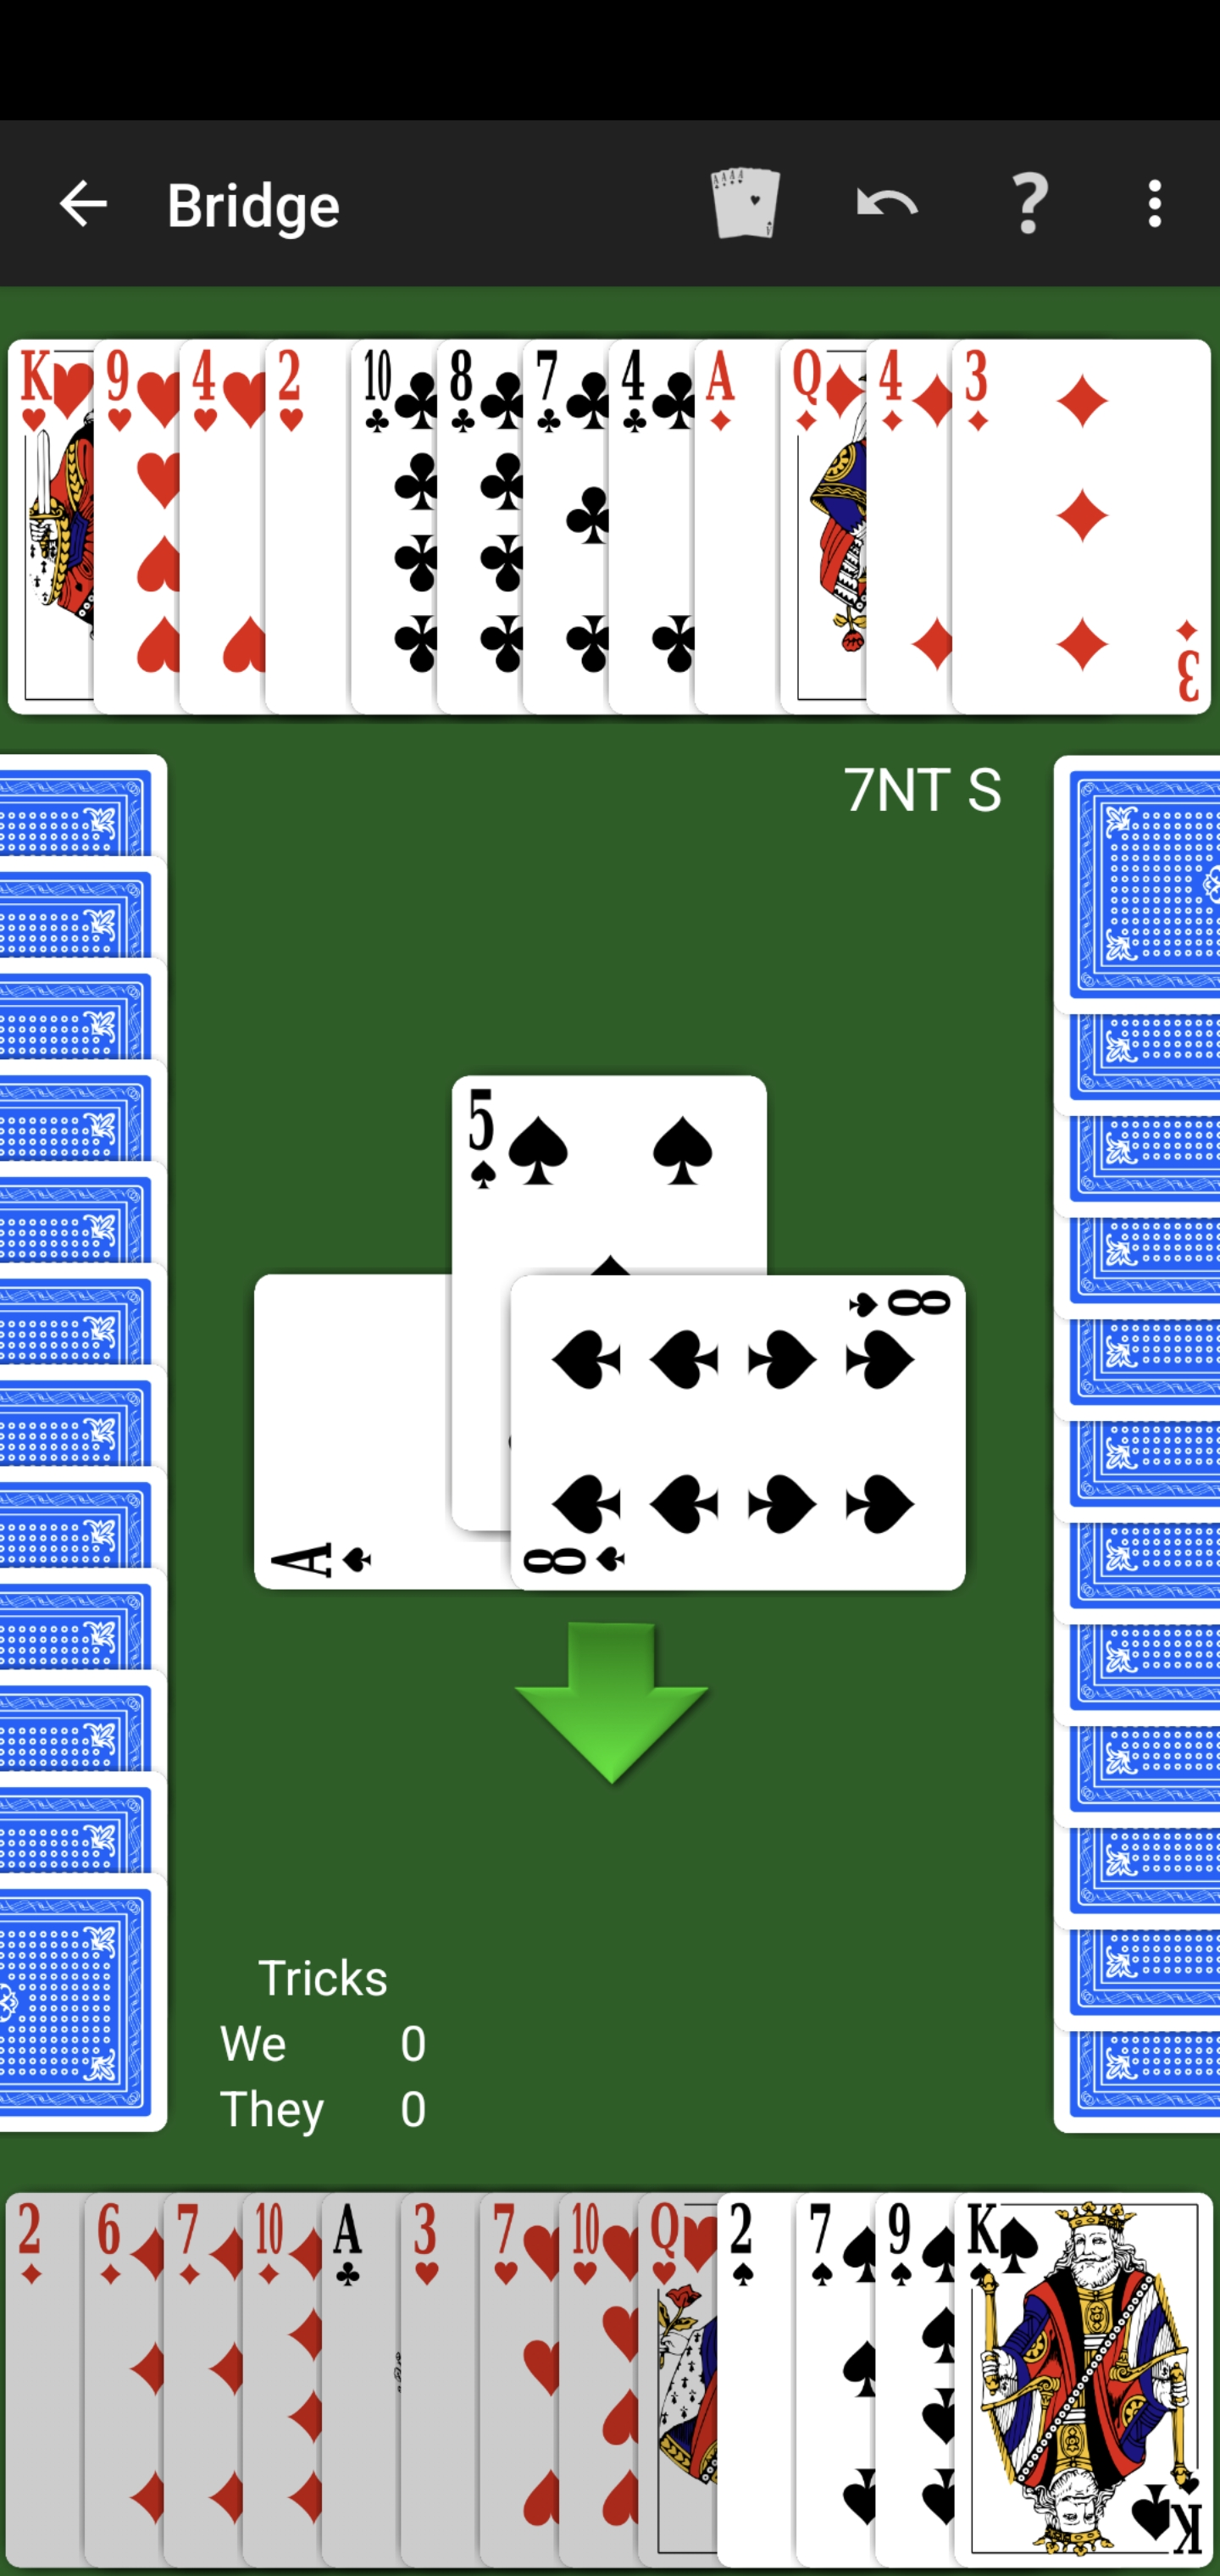
\includegraphics[width=.4\textwidth]{img/brydz-platformy/neuralplay1.jpg}
        \label{fig:neural-play-1}
    }%
    \hspace*{0.5cm}
    \subfloat[Historia bieżącej rozgrywki]{
        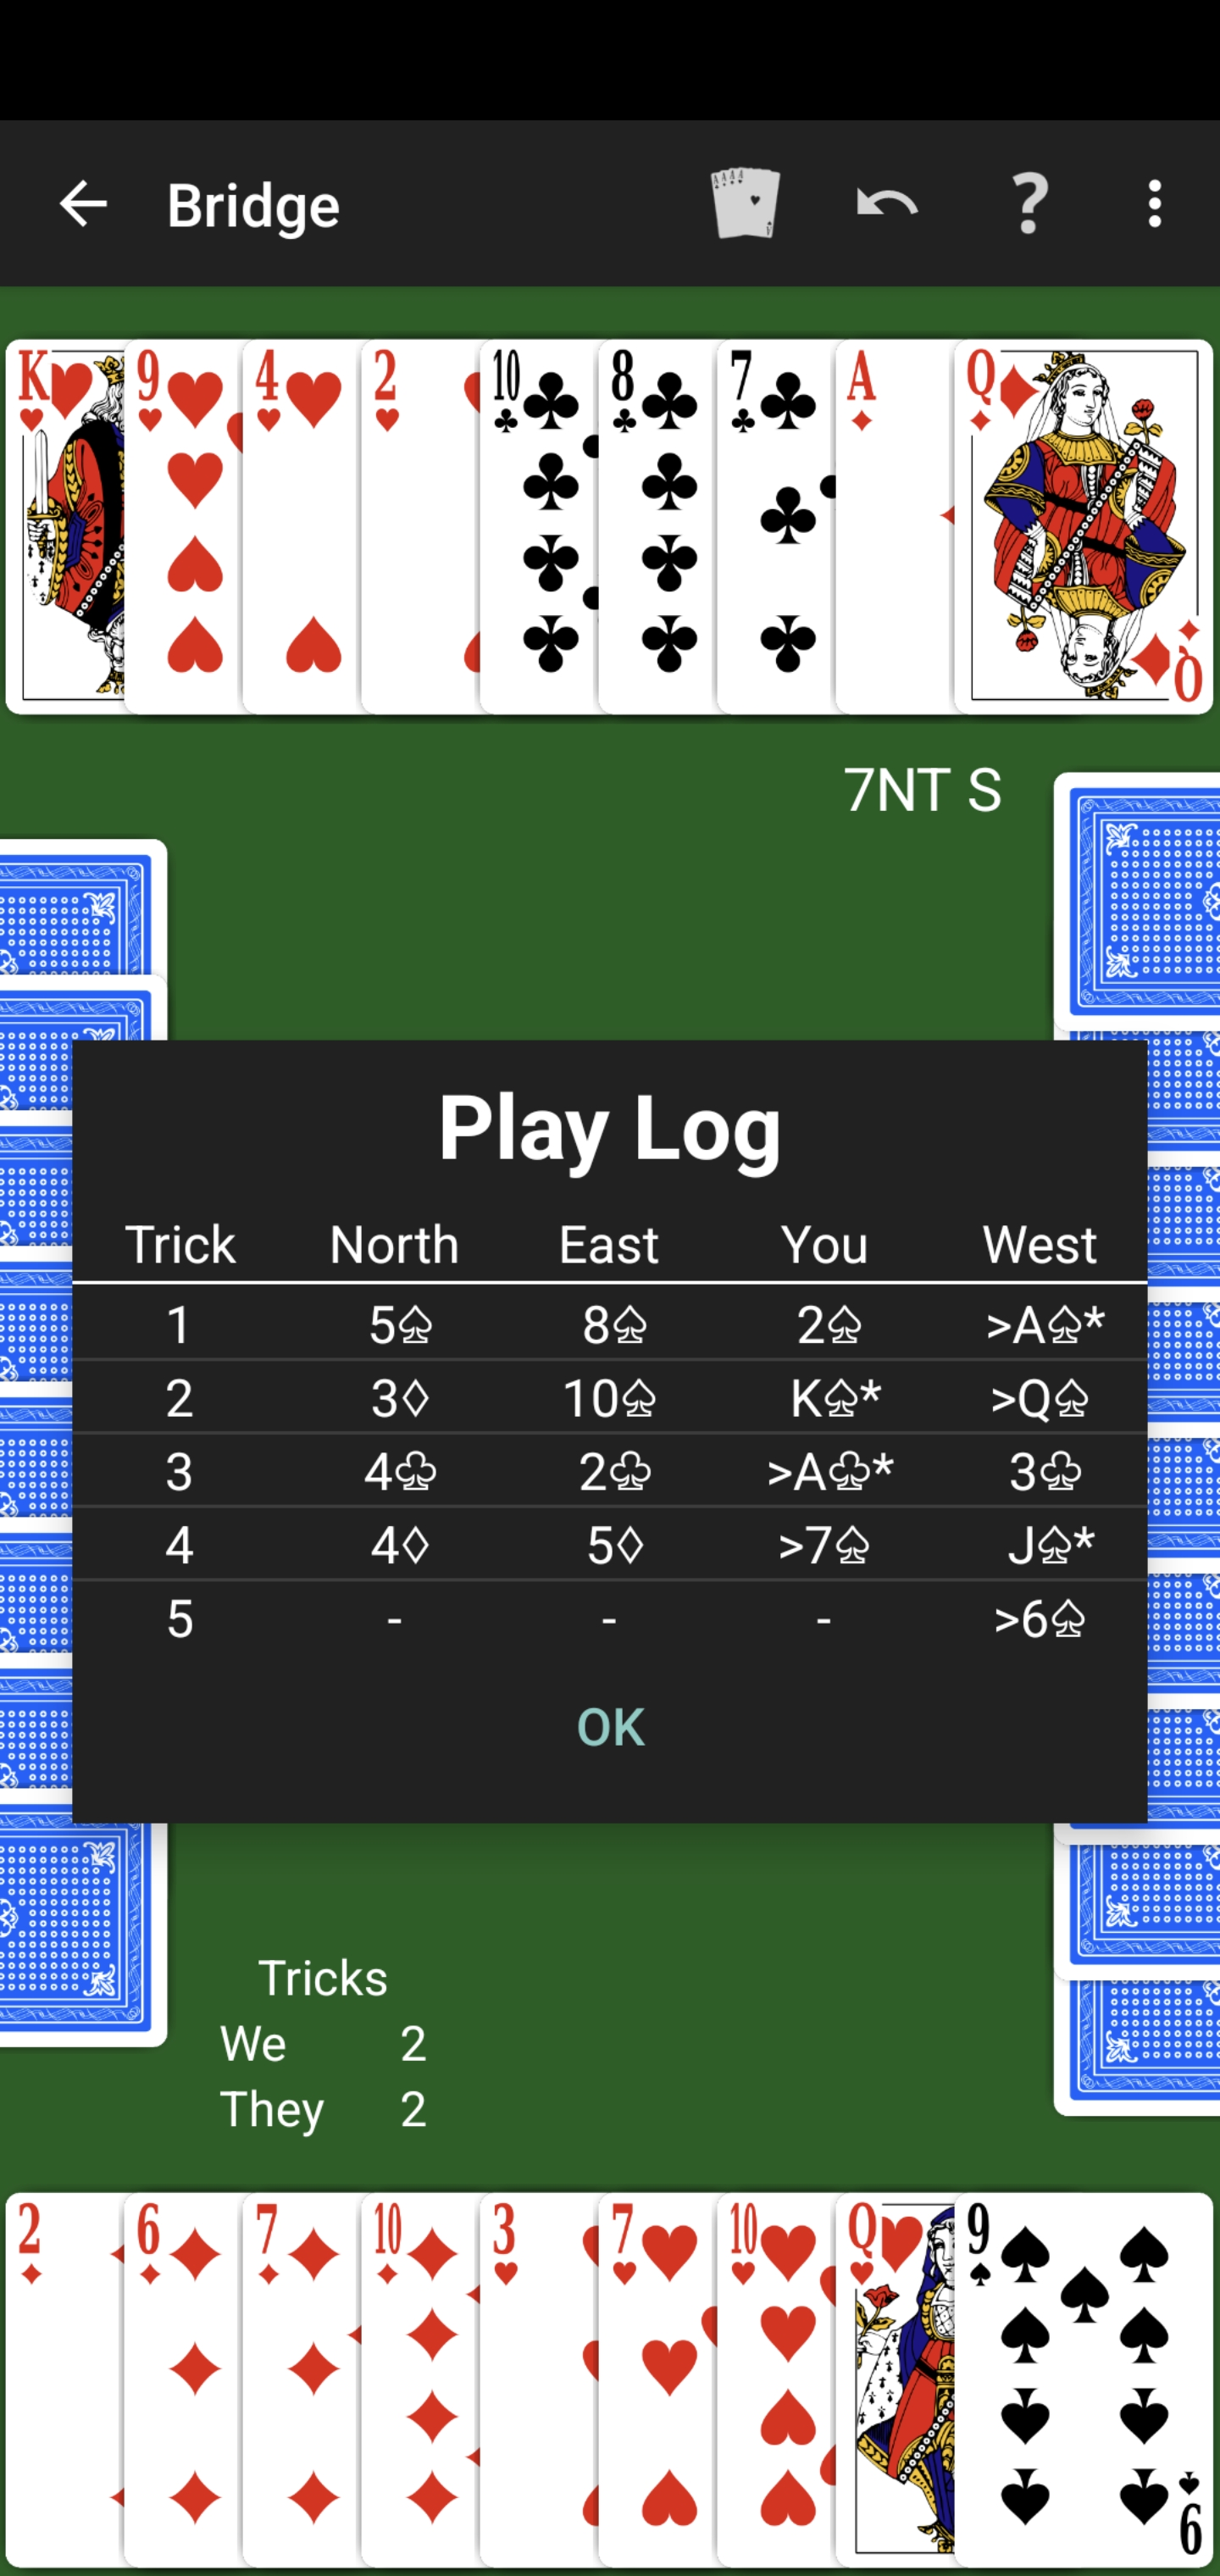
\includegraphics[width=.4\textwidth]{img/brydz-platformy/neuralplay2.jpg}
        \label{fig:neural-play-2}
    }%
    \caption{Rozgrywka brydża w aplikacji Bridge by NeuralPlay}
    \label{fig:neural-play}
\end{figure}

Wirtualny asystent może stanowić rozwiązanie dla tych problemów. Poprzez
zintegrowanie sztucznej inteligencji z~brydżem, aplikacja będzie w~stanie
zapewnić użytkownikom możliwość
rozgrywania partii z~wirtualnym partnerem, który będzie reagował na decyzje
gracza i~pomagał mu w~rozwijaniu jego umiejętności.

Dzięki temu projektowi, użytkownicy będą mieli możliwość prostszego i~bardziej
efektywnego nauczania się gry w~brydża. Lepszy dostęp odpowiednich partnerów
do gry pozwoli na intensywny i~satysfakcjonujący rozwój ich
umiejętności oraz~pasji. Asystent umożliwi naukę
i~doskonalenie umiejętności w~grze, a~także będzie w~stanie dostosować
się do odpowiedniego poziomu wybranego przez użytkownika.
\newline

Obecnie na rynku istnieje kilka analogicznych rozwiązań, jak na przykład
aplikacje internetowe Funbridge \cite{funbridge}, Bridge Base \cite{bridgebase},
BridgeAce+ \cite{bridgeace} oraz mobilna wersja Bridge by NeuralPlay
\cite{neuralplay}. W~przypadku BridgeAce+, użytkownik może korzystać wyłącznie
z~opcji nauki brydża w pojedynkę, gdzie partnerem i~przeciwnikami są boty
wykorzystujące sztuczną inteligencję. Natomiast Funbridge pozwala graczom
rywalizować ze sobą przez Internet oraz uczyć się grając z~botem oraz
przechodząc kursy. Po zakończeniu rozgrywki, użytkownik może przeanalizować
swoje błędy, jednak dostęp do tej opcji wymaga wykupienia konta premium.
Bridge Base oferuje wiele trybów gry, zarówno przeciwko botom jak i~innym
użytkownikom, jednak jego minus stanowi mało intuicyjny interfejs graficzny
Rys.~\ref{fig:bridge-base}. Aplikacja NeuralPlay oferuje pełną rozgrywkę w~brydża
z~wykorzystaniem zaprojektowanego AI, które zna wybrane metody licytowania.
Niestety, nawet rozgrywka przeciwko najtrudniejszemu poziomowi sztucznej
inteligencji, może być wygrana przez osobę mało doświadczoną.
\newline

Jak można zauważyć, istnieją już dostępne aplikacje umożliwiające naukę
i~grę w brydża, jednak mają one istotne wady. Brakuje rozwiązania, które
byłoby dostępne bez konieczności ponoszenia kosztów, umożliwiało naukę
i~rywalizację z~innymi użytkownikami oraz posiadało intuicyjny i~przyjazny
interfejs graficzny. Naszym celem jest połączenie większości tych funkcji
w~naszej własnej aplikacji.



\FloatBarrier

\section{Wizja produktu}

Produkt będzie aplikacją webową umożliwiająca grę w~brydża,
bez konieczności posiadania znajomych do gry.
Partnera lub przeciwnika będzie mógł zastąpić wirtualny asystent.
Jego zadaniem jest zapewnienie odpowiedniego
dla użytkownika towarzysza, którego poziom jest zależny od wybranej
preferencji. Użytkownicy będą mogli dostosować trudność, aby asystent osiągnął
planowane przez nich cele, takie jak nauka, rozgrywka na podobnym poziomie
lub zostać wyzwaniem dla doświadczonych zawodników.

Aplikacja będzie również umożliwiała grę w~brydża z~udziałem jednego lub więcej użytkowników,
którzy będą mogli połączyć się przez Internet, dzięki centralnemu serwerowi.
Zamierzane jest zaprojektowanie jej w~taki sposób, aby była intuicyjna i~łatwa
w~obsłudze dla wszystkich użytkowników, zarówno początkujących, jak
i~doświadczonych.

%%%

\section{Stos technologiczny}

Aplikacja internetowa zostanie napisana w~frameworku React \cite{React}.
Zdecydowaliśmy się na ten wybór, ze względu na dużą popularność tej
technologii. W~2022 roku serwis Stack Overflow \cite{StackOverflow} przeprowadził ankietę dotyczącą między innymi wykorzystywanych technologii
webowych \cite{React-stack}. Aż 42.62\% respondentów wybrało React,
zajmując 2 miejsce w~rankingu. Jako że wykorzystuje on język Javascript,
który według wspomnianej ankiety jest najpopularniejszym językiem programowania,
dostępna jest olbrzymia baza bibliotek i~sprawdzonych rozwiązań. Za wizualną
część projektu będzie odpowiedzialny framework Tailwind CSS \cite{Tailwind}.
Oferuje on gotowe klasy CSS, które pozwalają na szybkie tworzenie responsywnych
i~estetycznych interfejsów. Część serwerowa obsługująca sesje gier zostanie
napisana w~języku Python \cite{Python} za pomocą biblioteki FastAPI
\cite{FastAPI}. Funkcjonalność związana z~obsługą użytkowników i~gromadzenia
danych będzie wykorzystywała usługę Google Firebase \cite{Firebase}.

Wirtualny asystent zostanie zrealizowany jako osobna biblioteka udostępniająca
własne API. Backend obsługujący sesje gier, po dołączeniu biblioteki asystenta,
będzie mógł wysłać do API asystenta aktualny stan gry, aby otrzymać
odpowiedź zawierającą analizę tego stanu, między innymi
prawdopodobieństwo wygrania każdej z~par graczy oraz listę
najlepszych ruchów, jakie mogą być wykonane przez następnego gracza.

Na podstawie wstępnych badań, wybrane zostało 5~algorytmów AI,
które będą rozważane do zastosowania w~projekcie asystenta.
W~kolejności od najbardziej złożonego do
najprostszego w implementacji są to:
\begin{enumerate}
    \item \textbf{Algorytm Regularized Nash Dynamics \cite{doi:10.1126/science.add4679}}\\
          Algorytm oparty na teorii gier, który wykorzystuje sieć neuronową do
          predykcji najlepszego ruchu. Istnieje dowód formalny, że algorytm
          zbiega do równowagi Nasha, czyli optymalnej strategii.

    \item \textbf{Algorytm AlphaZero \cite{AlphaZeroPaper} połączony z algorytmem IS-MCTS \cite{6203567}}\\
          Algorytm AlphaZero jest wariantem algorytmu Monte Carlo Tree Search,
          który wykorzystuje sieć neuronową do oceny stanu gry.
          Algorytm Information Set MCTS (IS-MCTS) jest modyfikacją algorytmu MCTS, która pozwala na
          przeszukiwanie drzewa stanów gry o~niepełnej informacji.
          Możliwe jest połączenie tych dwóch algorytmów, aby uzyskać
          Information Set AlphaZero.

    \item \textbf{Implementacja algorytmu IS-MCTS z biblioteki OpenSpiel \cite{LanctotEtAl2019OpenSpiel}}\\
          Biblioteka OpenSpiel zawiera implementację algorytmu IS-MCTS,
          który może być wykorzystany do gry w~brydża.

    \item \textbf{Program AI do brydża GIB \cite{Ginsberg1999GIBST}}\\
          GIB jest jednym ze starszych programów AI do brydża. Możliwe jest
          jego bezpośrednie wykorzystanie w~projekcie.

    \item \textbf{Algorytm Pure Monte Carlo Tree Search \cite{pmcts}}\\
          Algorytm równoważny MCTS dla maksymalnej głębokości drzewa równej 1.
\end{enumerate}


%%%

\section{Analiza zagrożeń}
\label{sec:analiza_zagrozen}

Gra w~brydża jest jedną z~najtrudniejszych gier strategicznych na świecie.
Do tej pory nie powstał żaden system AI grający na mistrzowskim poziomie
uwzględniający pełną wersję gry z~licytacją \cite{Bethe2021AdvancesIC}.
Implementacja gracza AI o~wystarczająco wysokim poziomie umiejętności może
być znacznym wyzwaniem. W~literaturze zostało opisane wiele metod AI do brydża
\cite{Zhang2019DesignAD,Zhang2022TheSO,Zhang2022AIEB,Ginsberg1999GIBST}
co sugeruje, że jest to temat dalej otwarty i~ciągle rozwijany.
Przedstawiliśmy 5~różnych możliwości implementacji AI.
W~razie problemów z~implementacją jednej z~nich, pozostałe
zostaną wykorzystane jako plany awaryjne.

Ważnym elementem każdej gry online jest niezawodność systemu
backend oraz jego odporność na awarie.
Aplikacja musi być również odporna na problemy sieciowe.
Platforma Firebase zapewnia nam mechanizmy zabezpieczające
przed problemami po stronie klienta, połączenia internetowego
oraz samego backendu Firebase, który jest redundantnie
rozproszony po całym świecie.
Samo hostowanie strony internetowej zostanie zrealizowane
usługą Firebase Hosting, która również zapewnia wysoką
niezawodność.
Bezpieczeństwo aplikacji będzie zarządzane za pomocą
usługi Firebase Authentication.

Powyżej wymienione usługi są dostępne w darmowym planie.
Podczas pracy nad projektem może dojść do sytuacji, że
zostaną one przekształcone w~plan płatny.
Jeśli dostępne platformy chmurowe staną się niedostępne,
zastosowany zostanie własny serwer działający
w~oparciu o~komputer osobisty lub mikrokomputer, np. Raspberry Pi \cite{RPi}.

% needs latex magic
\begin{table}[h]
    \centering
    \begin{tabularx}{\textwidth}{|p{5.5cm}|Y|Y|}
        \hline
        \textbf{Zagrożenie}                                    & \textbf{Prawdopodobieństwo wystąpienia} & \textbf{Zagrożenie dla projektu} \tabularnewline[0.2cm]
        \hline
        Problemy w implementacji AI                            & Wysokie                                 & Średnie (podano plany awaryjne)  \tabularnewline[0.2cm]
        Nie osiągniecie poziomu mistrzowskiego przez asystenta & Wysokie                                 & Niskie                           \tabularnewline[0.3cm]
        Niska niezawodność produktu                            & Niskie                                  & Średnie                          \tabularnewline[0.1cm]
        Niska niezawodność produktu                            & Niskie                                  & Średnie                          \tabularnewline[0.1cm]
        \hline
    \end{tabularx}
    \caption{Analiza zagrożeń}
    \label{tab:zagrozenia}
\end{table}

%%%

\newpage

\section{Szkic aplikacji}

Zostały przygotowane szkice interfejsu aplikacji
(Rys.~\ref{fig:figma_login}--\ref{fig:figma_game}).

\begin{figure}[h!]
    \centering
    \subfloat[Ekran logowania]{
        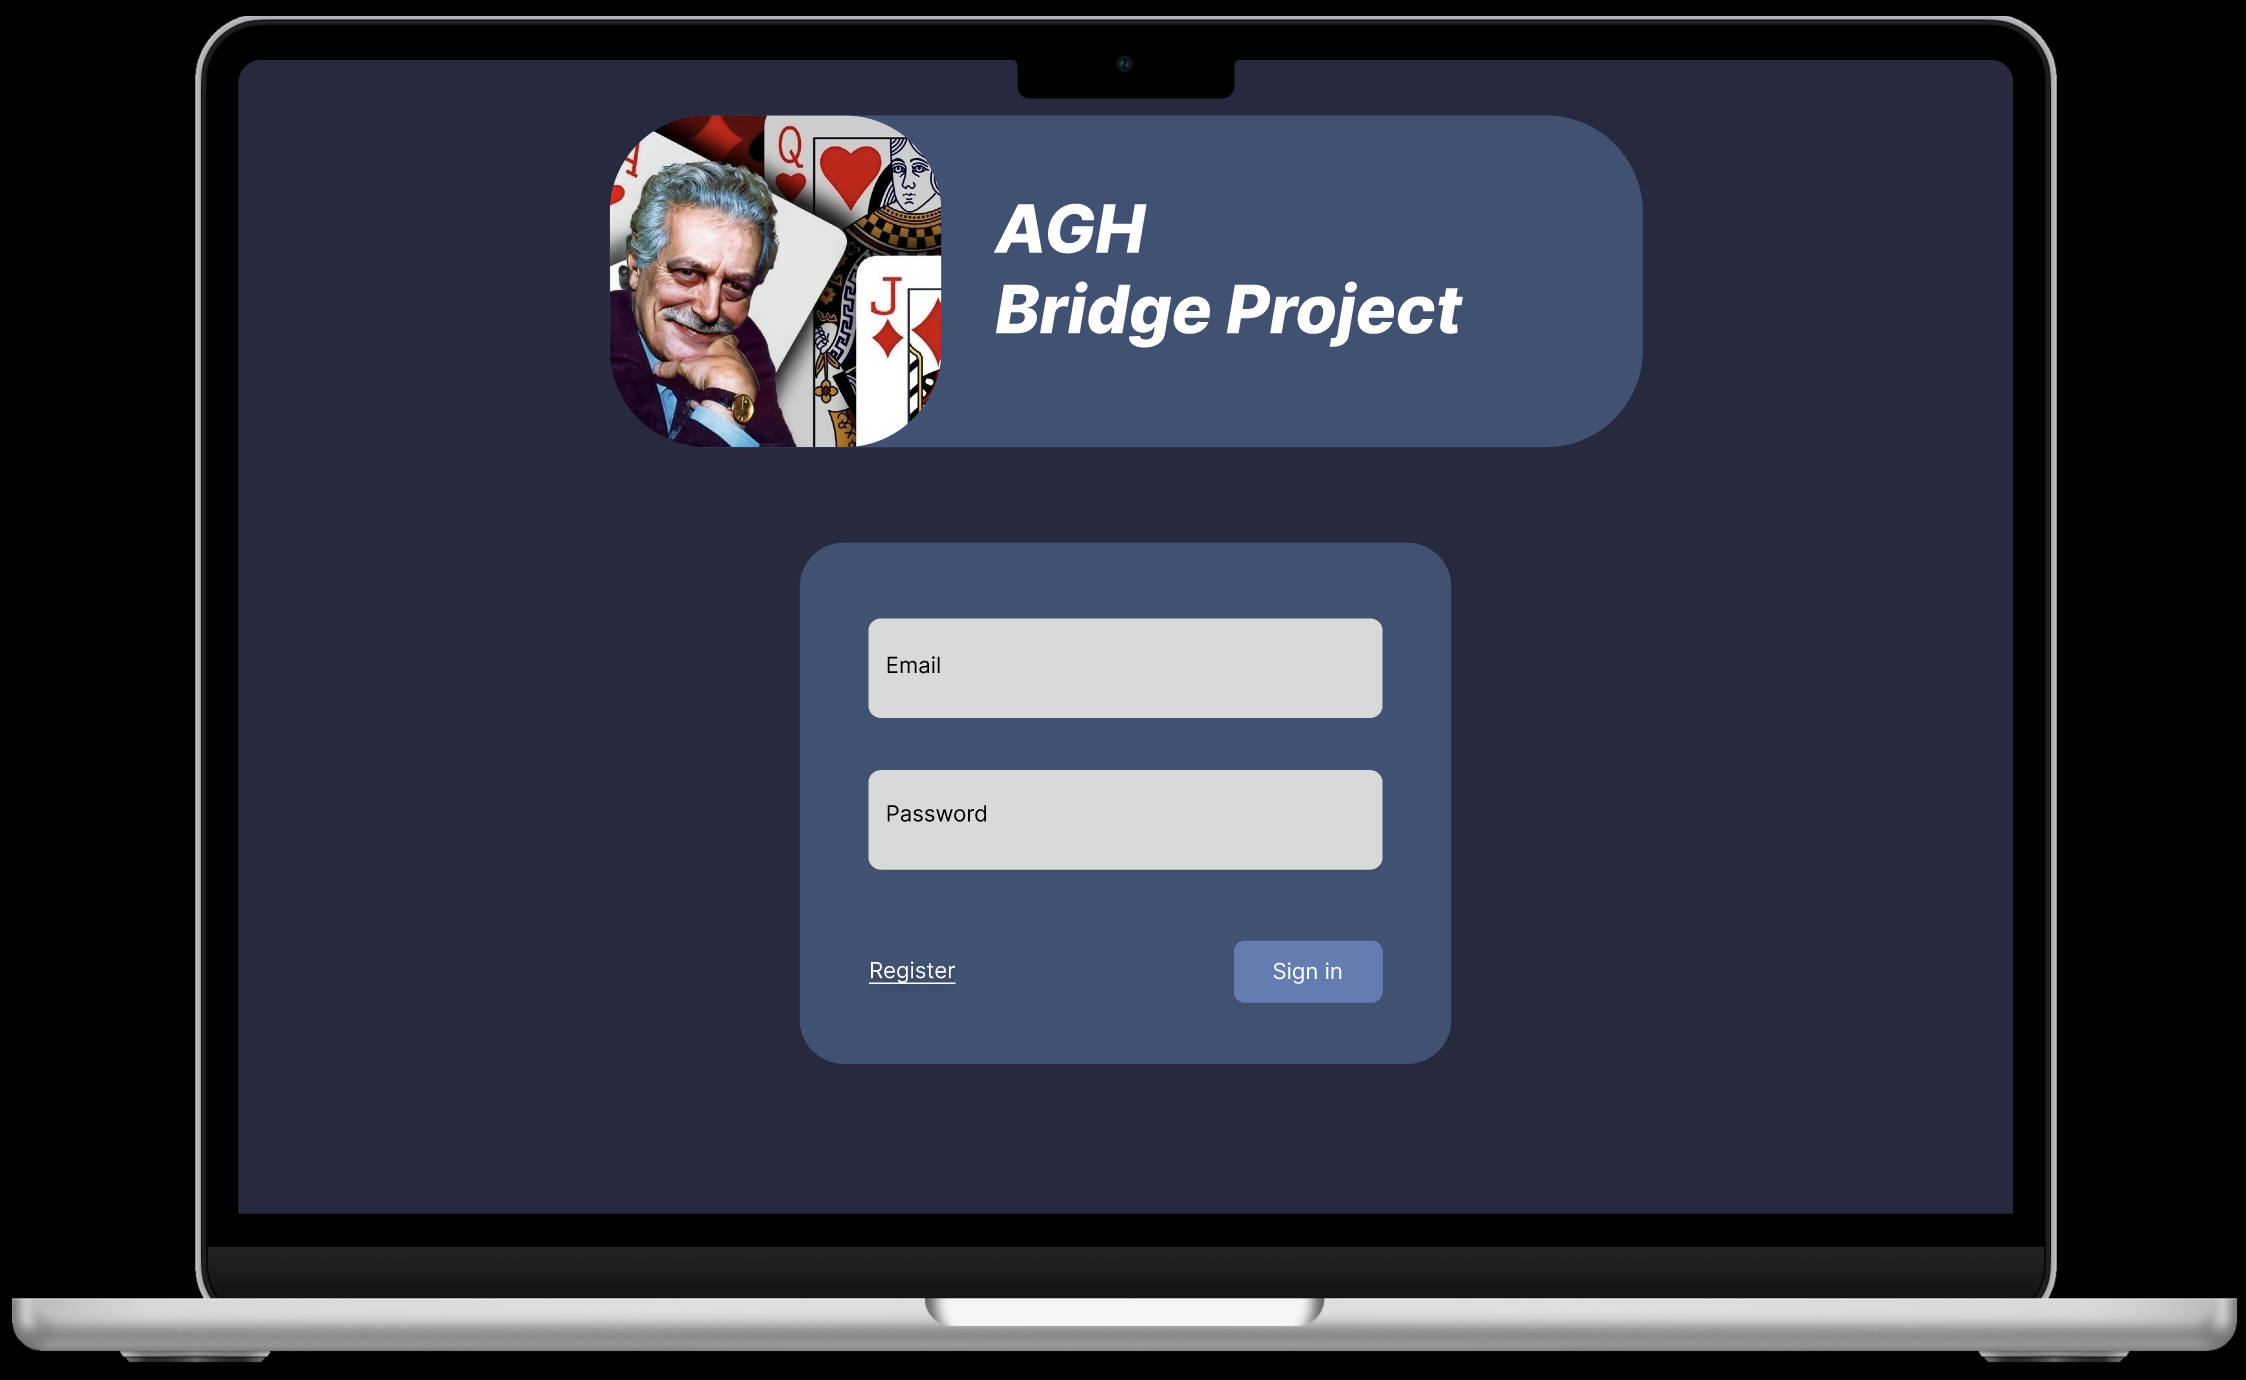
\includegraphics[width=0.45\textwidth]{img/figma-szkic/1.png}
        \label{fig:figma_login}
    }%
    \hspace*{0.5cm}
    \subfloat[Ekran główny]{
        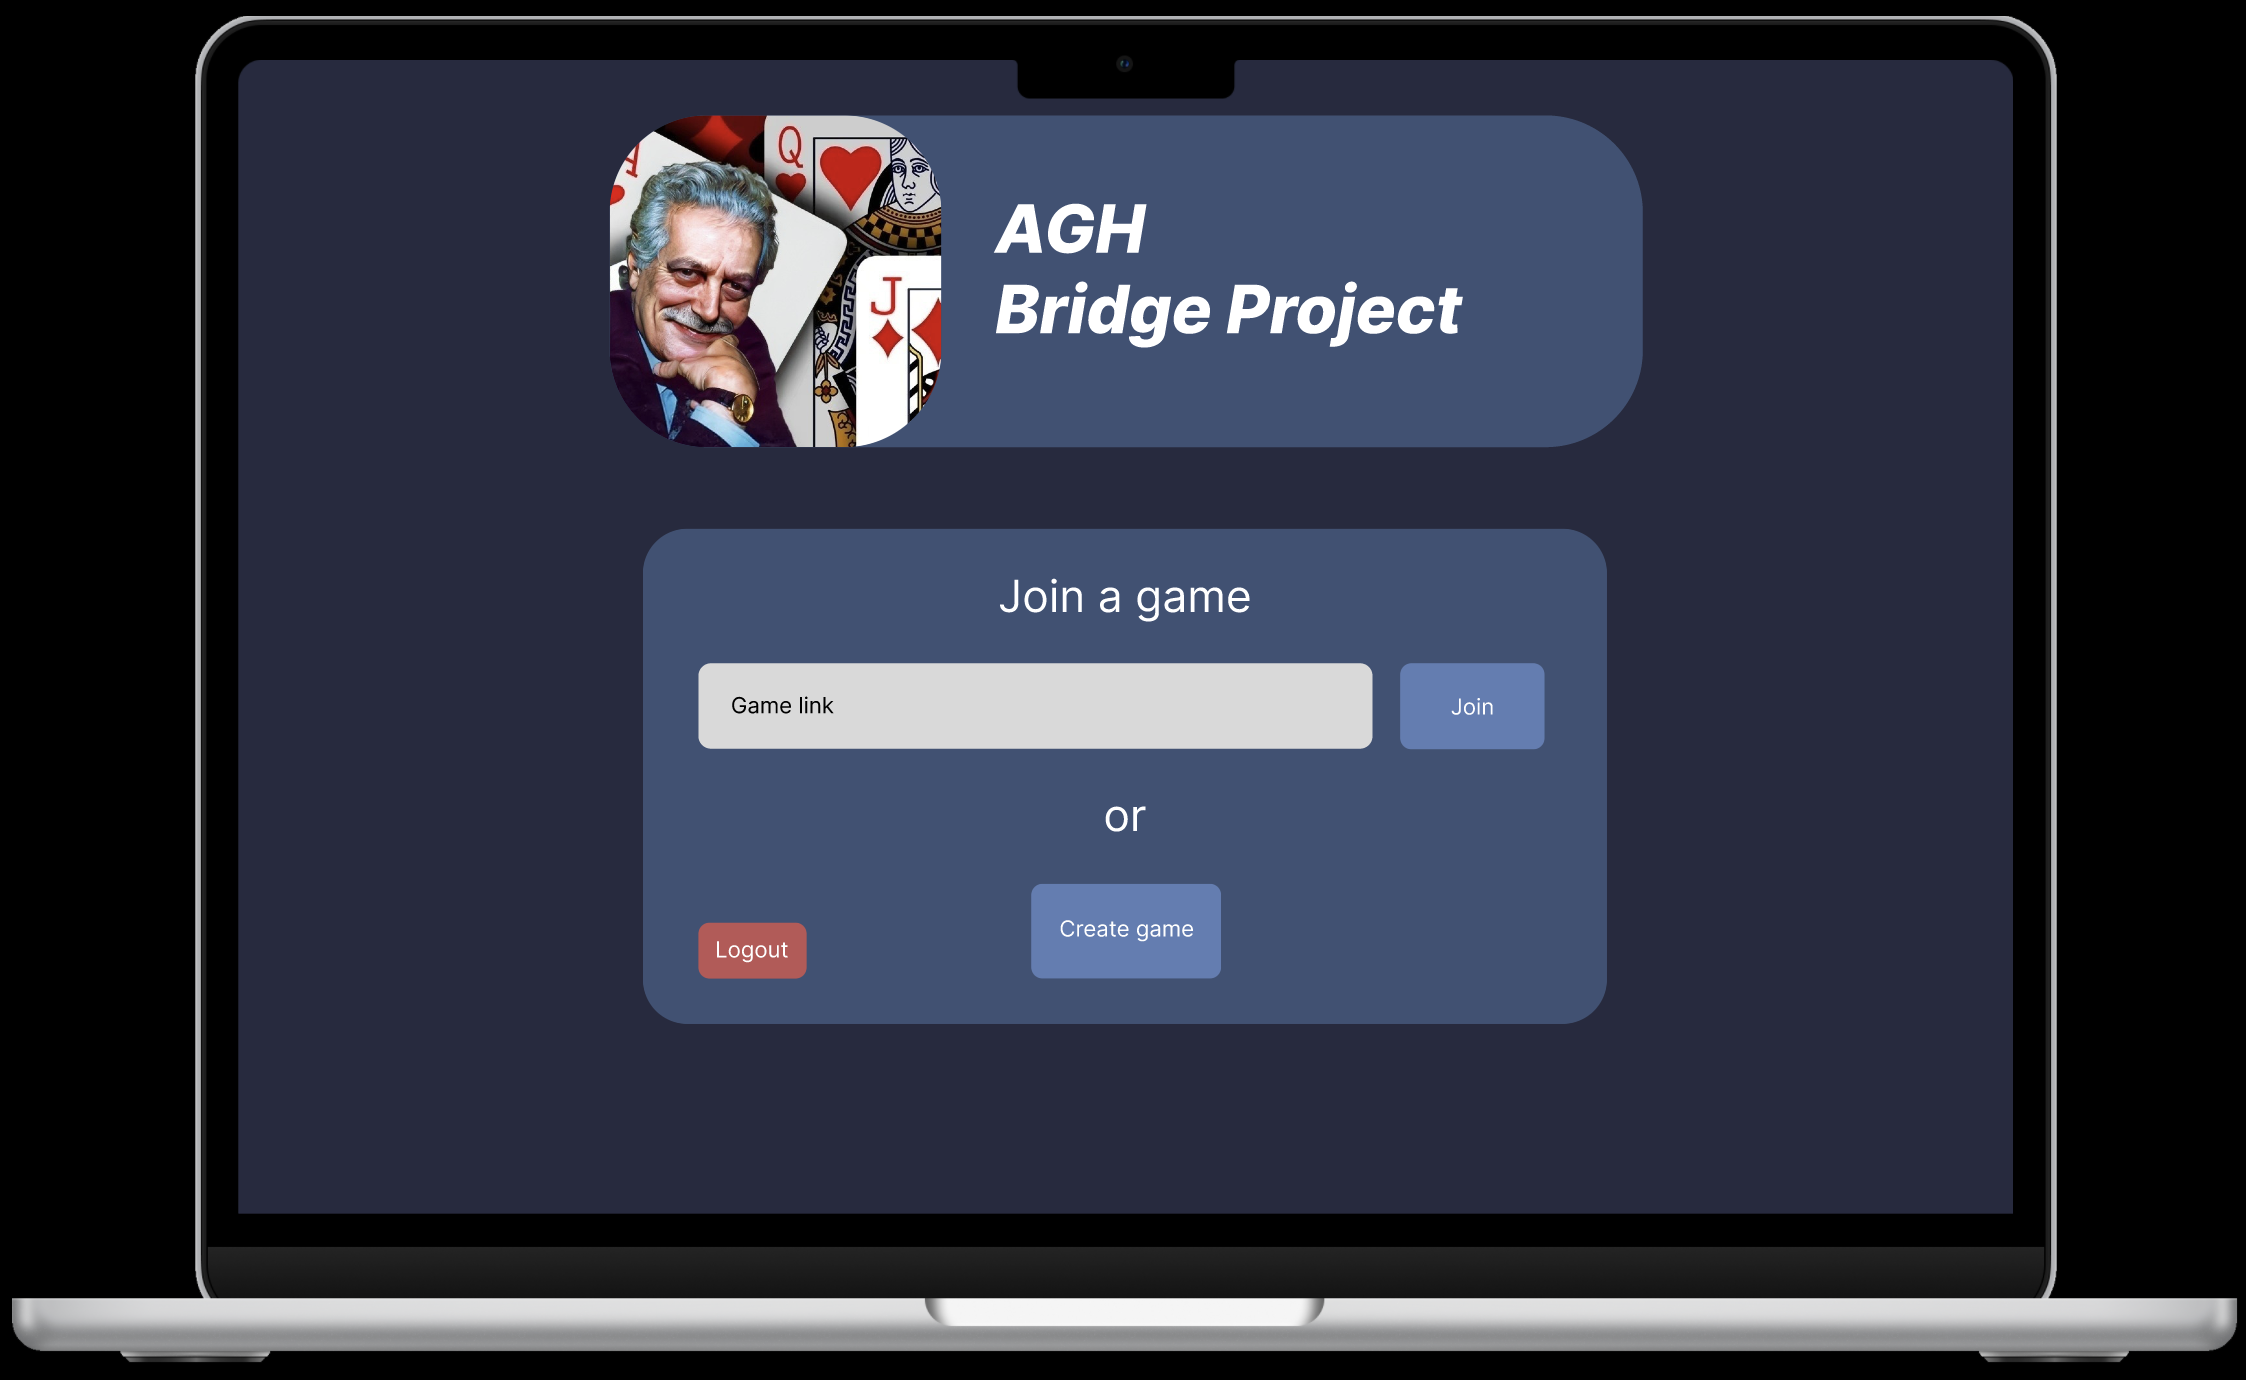
\includegraphics[width=0.45\textwidth]{img/figma-szkic/2.png}
    }%
    \\
    \subfloat[Ekran lobby]{
        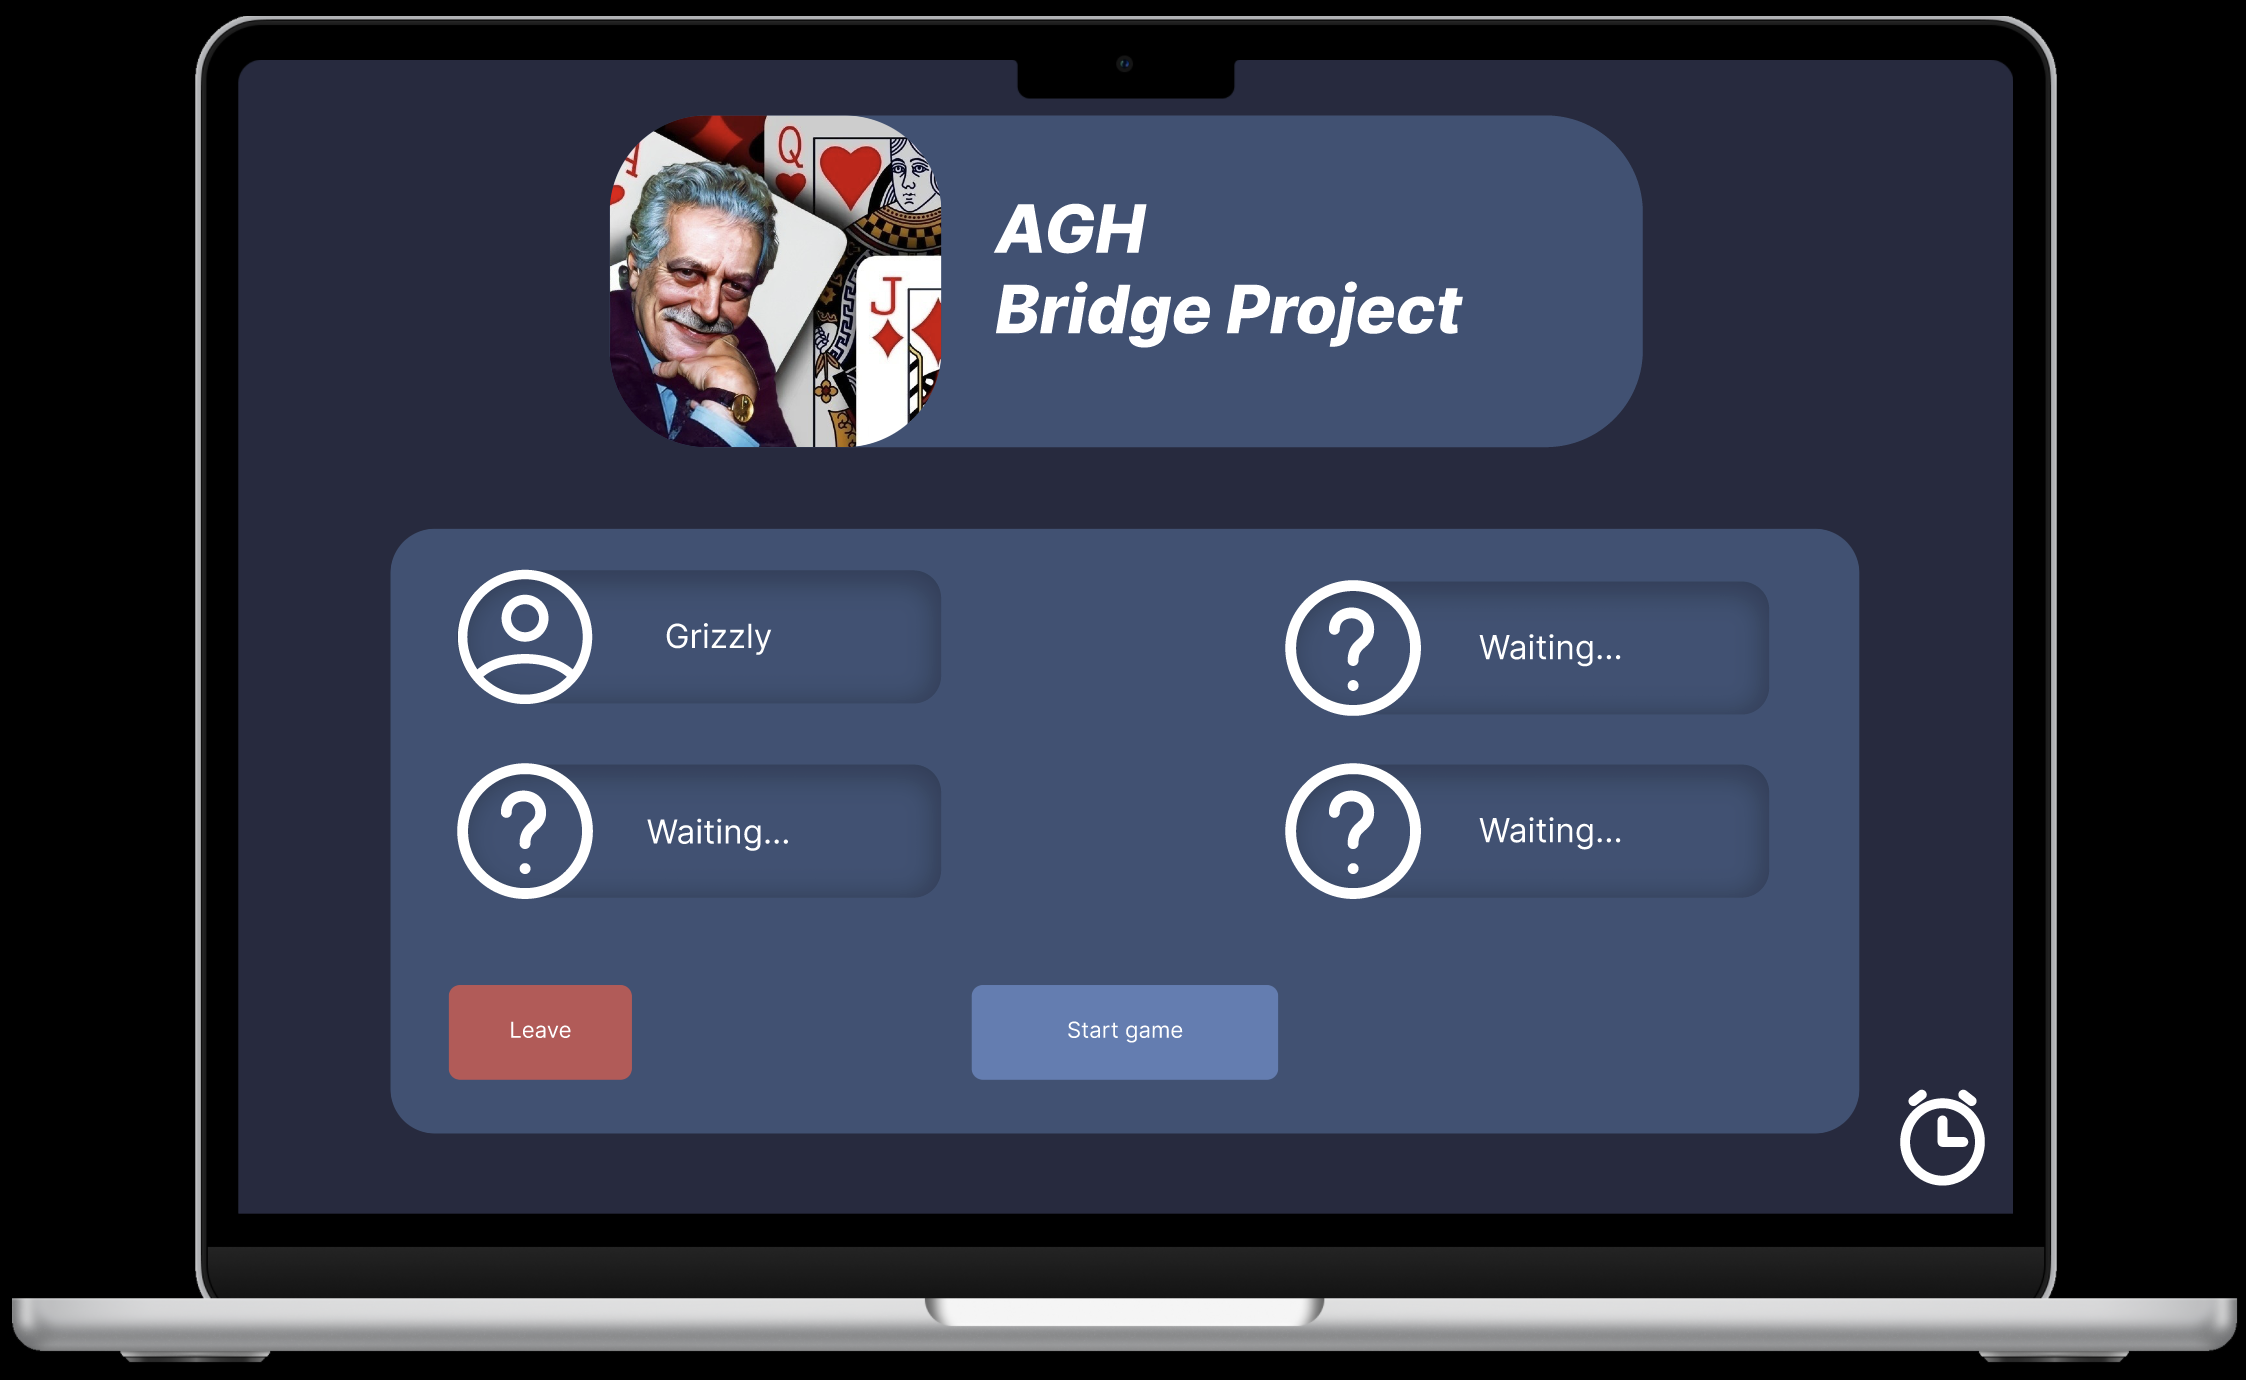
\includegraphics[width=0.45\textwidth]{img/figma-szkic/3.png}
    }%
    \hspace*{0.5cm}
    \subfloat[Ekran gry]{
        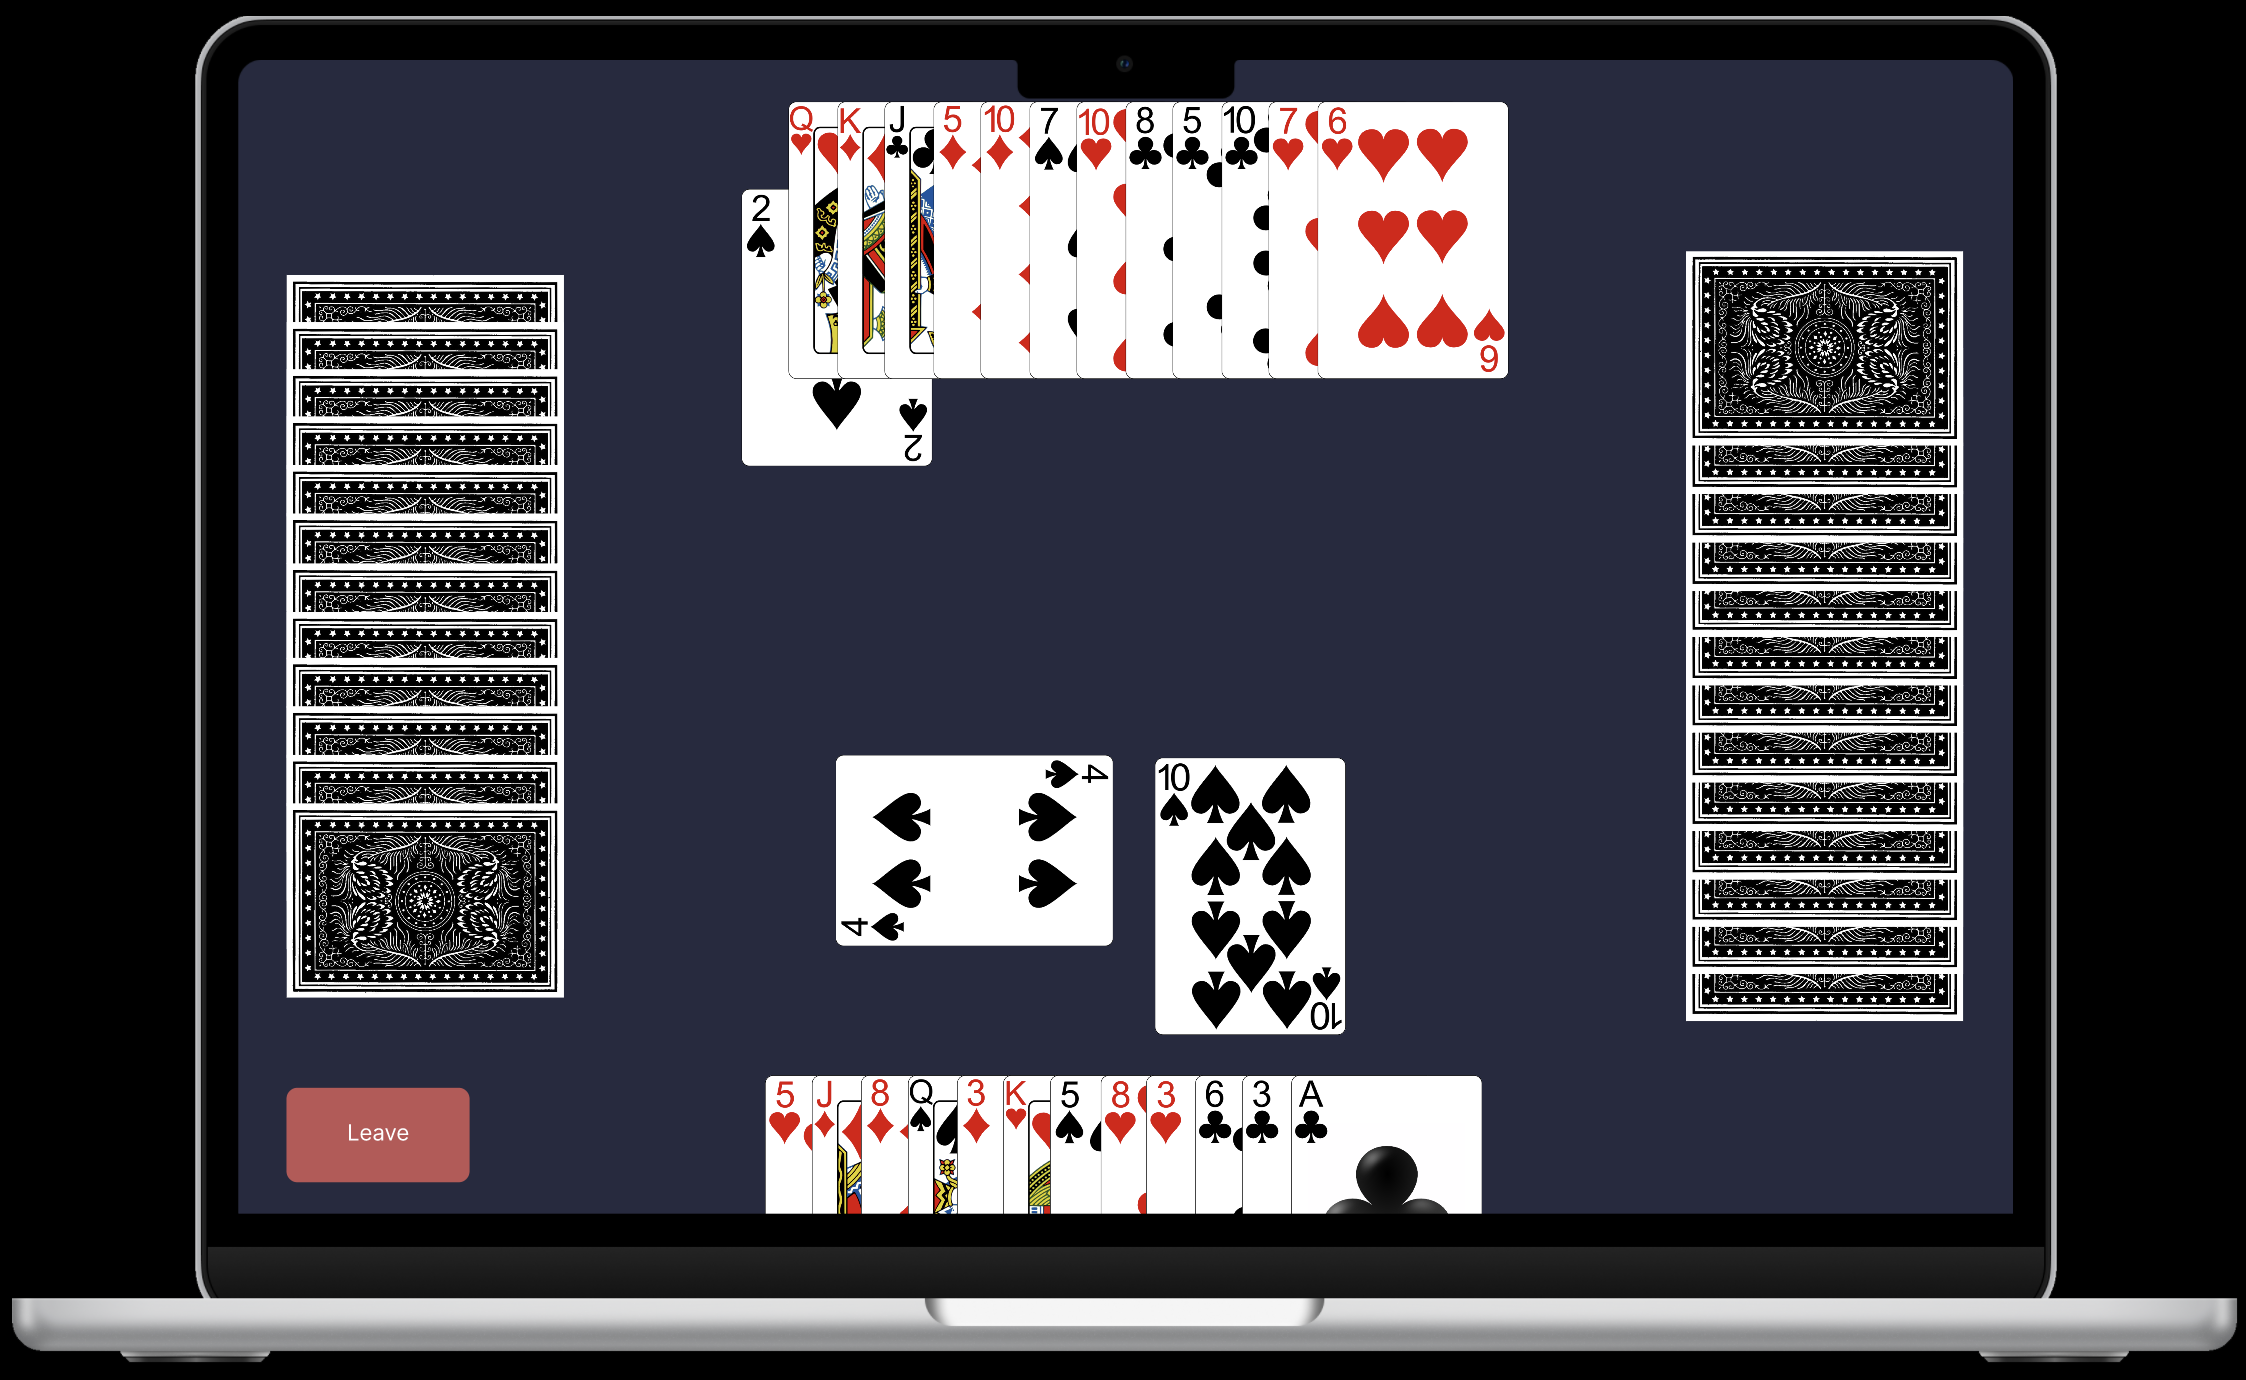
\includegraphics[width=0.45\textwidth]{img/figma-szkic/4.png}
        \label{fig:figma_game}
    }%
    \caption{Szkice interfejsu aplikacji}
\end{figure}

\FloatBarrier

\section{Słownik pojęć}

\begin{enumerate}
    \item Brydż -- karciana gra strategiczna rozgrywana przez dwie pary graczy,
    \item Użytkownik -- człowiek korzystający z aplikacji,
    \item Wirtualny asystent -- algorytm posiadający możliwość analizy rozgrywki w celu nauki, współpracy lub konkurencji z użytkownikiem,
    \item Gracz -- użytkownik lub wirtualny asystent biorący udział w rozgrywce,
    \item Partner -- drugi gracz grający w parze danego gracza,
    \item Przeciwnik -- jeden z graczy z pary grającej przeciwko danemu graczowi,
    \item Wirtualny partner -- partner będący wirtualnym asystentem,
    \item Wirtualny przeciwnik -- przeciwnik będący wirtualnym asystentem,
\end{enumerate}


\chapter{\ChapterTitleScope}
\label{sec:zakres-funkcjonalnosci}


\section{Kontekst użytkowania aplikacji}

Głównym zadaniem aplikacji jest zapewnienie użytkownikom platformy
umożliwiającej rozgrywkę w~brydża. Strona internetowa aplikacji jest
przystosowana do każdego rozmiaru ekranu, z~której mógłby korzystać
użytkownik. Dzięki temu można skorzystać z~aplikacji, wykorzystując
telefon, komputer stacjonarny, laptop lub nawet telewizor. Wymagany
jest tylko dostęp do Internetu.
%Aplikacja oprócz samej rozgrywki oferuje także przejrzenie
%wcześniejszych rozgrywek i~przeanalizowanie ich z~użyciem asystenta AI.

W~systemie aplikacji zdefiniowane są dwa typy użytkowników:
\begin{itemize}
  \item \textbf{zalogowany użytkownik} -- zalogowana osoba posiadająca konto w aplikacji, mająca dostęp do
        jej funkcjonalności,

  \item \textbf{anonimowy użytkownik} -- osoba niezalogowana, która nie
        posiada dostępu do
        % podstawowych
        funkcjonalności aplikacji.
        % Natomiast ma możliwość obserwowania trwających rozgrywek.
\end{itemize}

Funkcjonalności dostępne dla poszczególnych użytkowników:
\begin{itemize}
  \item \textbf{zalogowany użytkownik}:
        \begin{itemize}
          \item tworzenie i dołączanie do rozgrywek w brydża --
                gdy użytkownik założy lub zostanie jedynym
                użytkownikiem lobby, to staje się jego
                administratorem.
                Może zarządzać graczami znajdującymi się w~nim
                i~decydować ile graczy ma być zajęta przez asystenta AI.
          \item przeglądanie i analiza wcześniejszych rozgrywek
                z wykorzystaniem asystenta AI.
        \end{itemize}

  \item \textbf{anonimowy użytkownik}:
        \begin{itemize}
          \item obserwowanie trwających rozgrywek brydża.
        \end{itemize}
\end{itemize}

\begin{figure}[h]
  \centering
  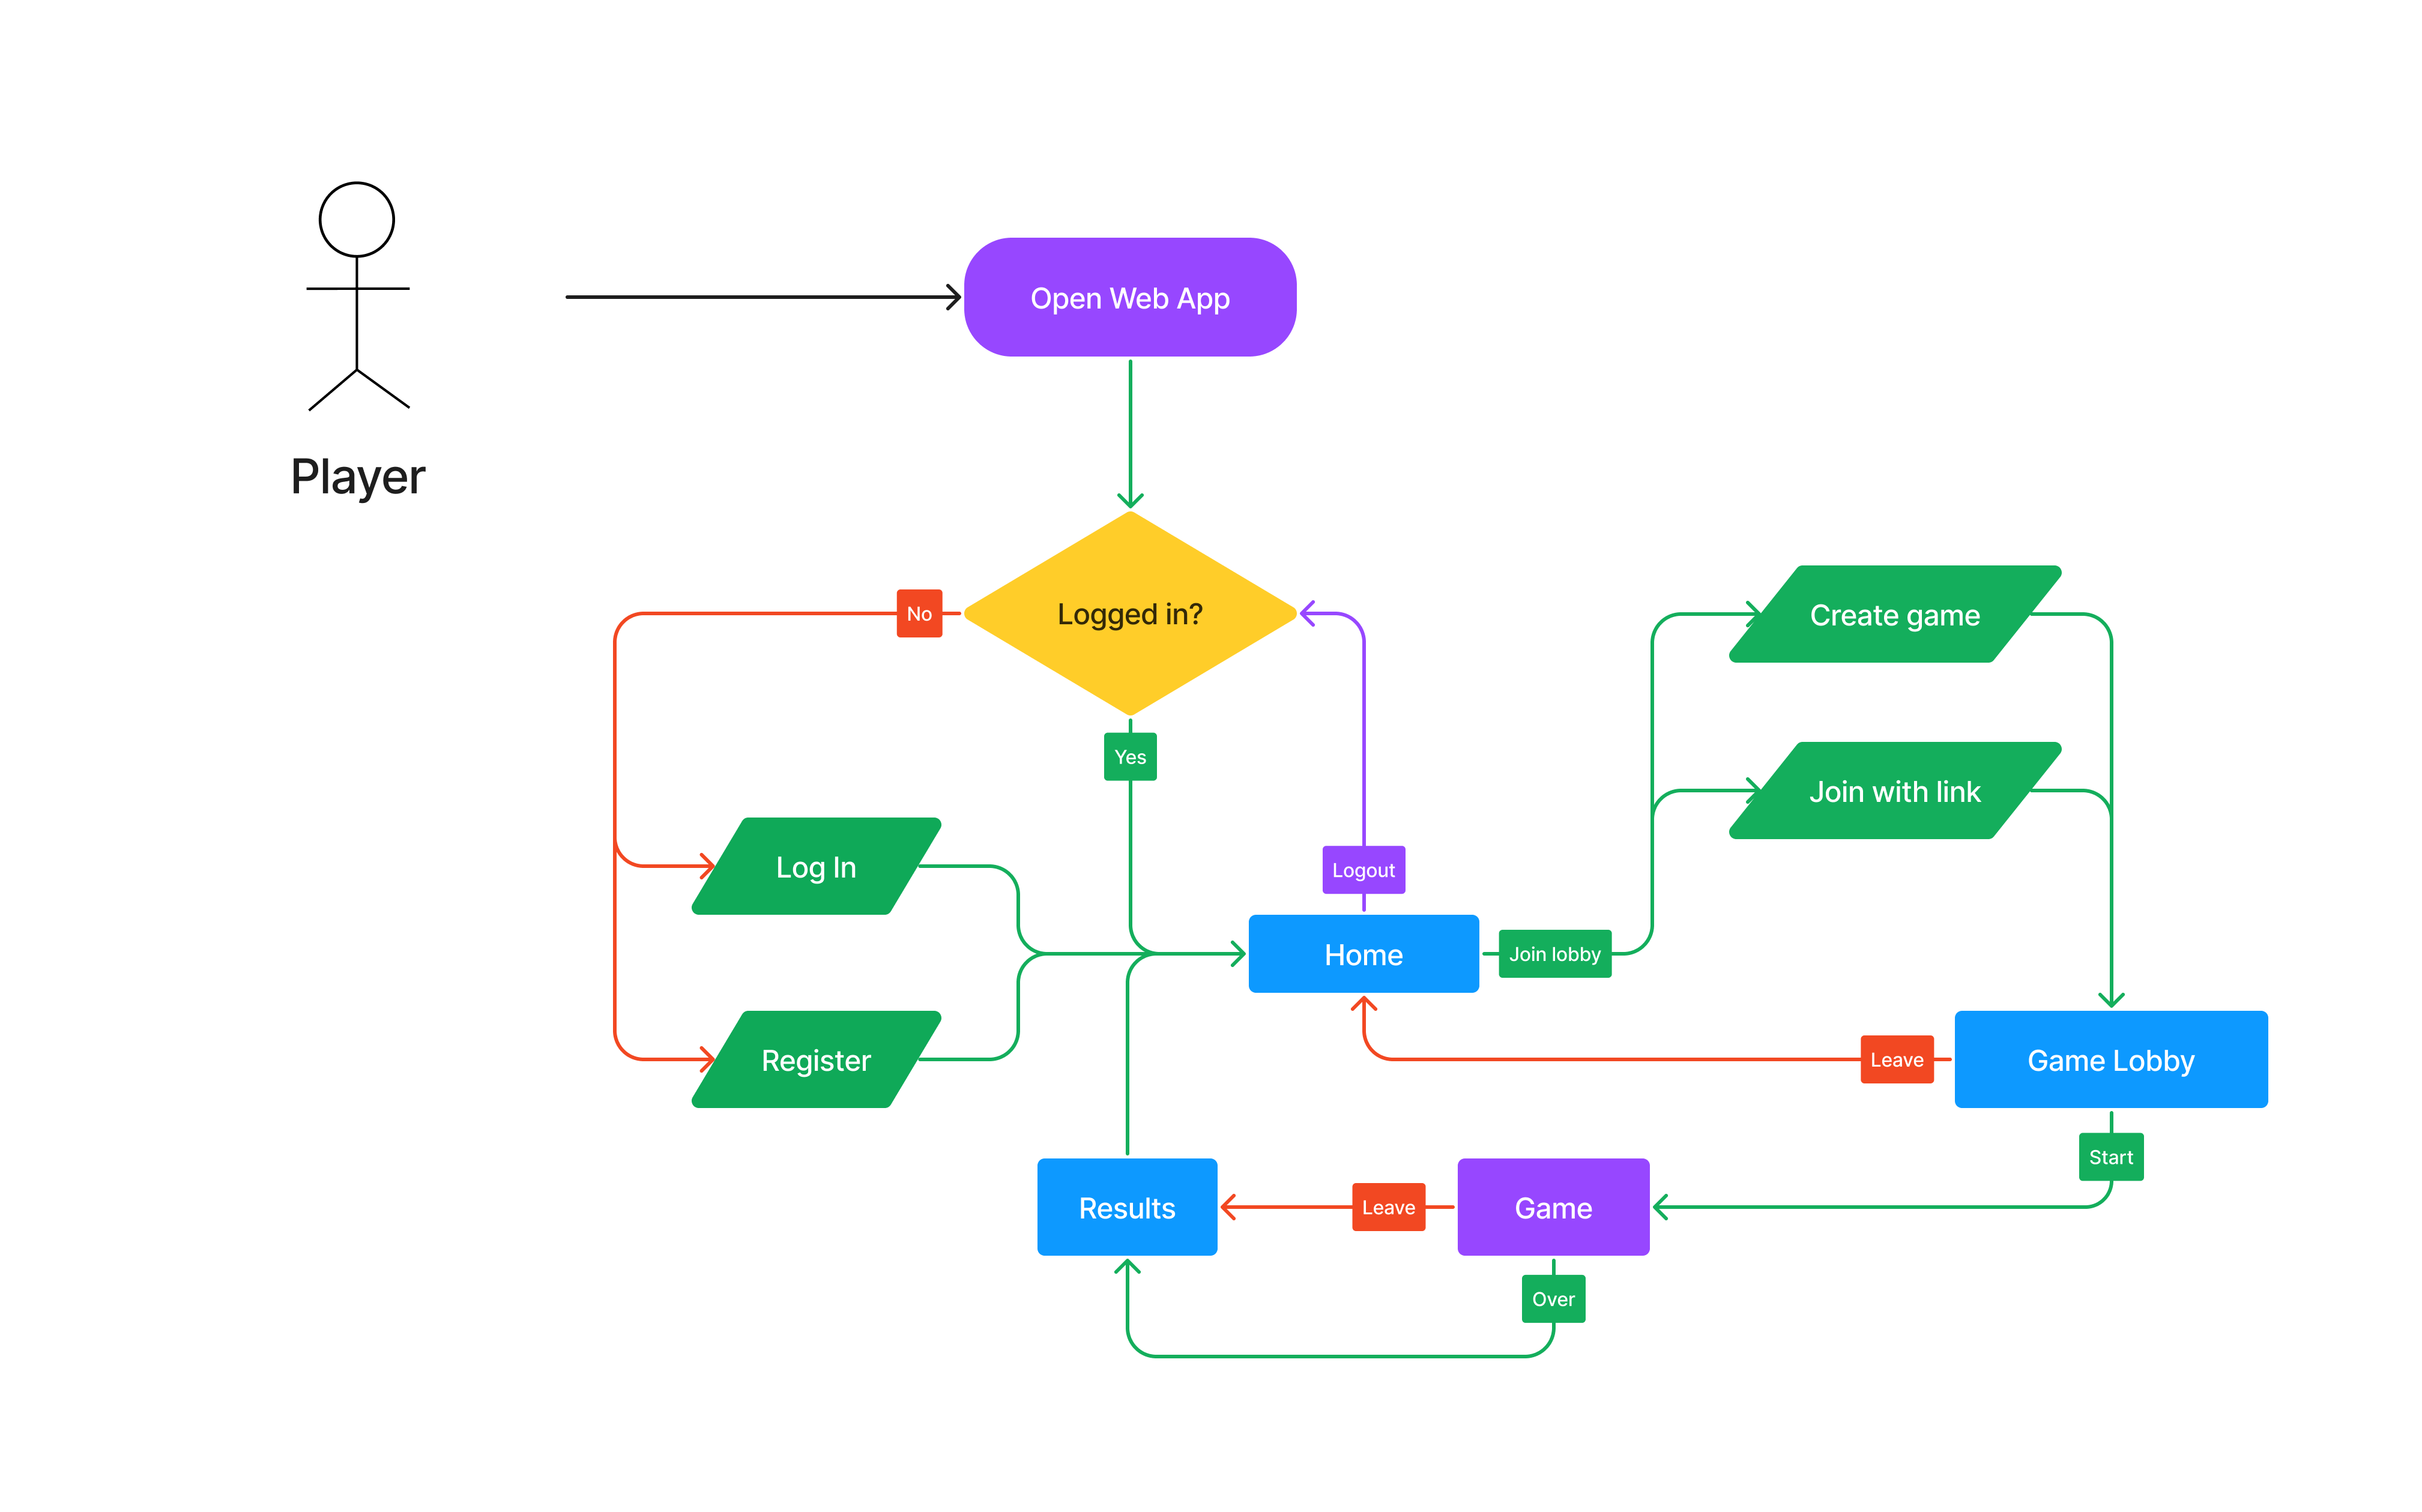
\includegraphics[width=\textwidth]{img/flow-aplikacji/user_flow.png}
  \caption{Schemat interakcji użytkownika z aplikacją}
\end{figure}

\begin{figure}[h]
  \centering
  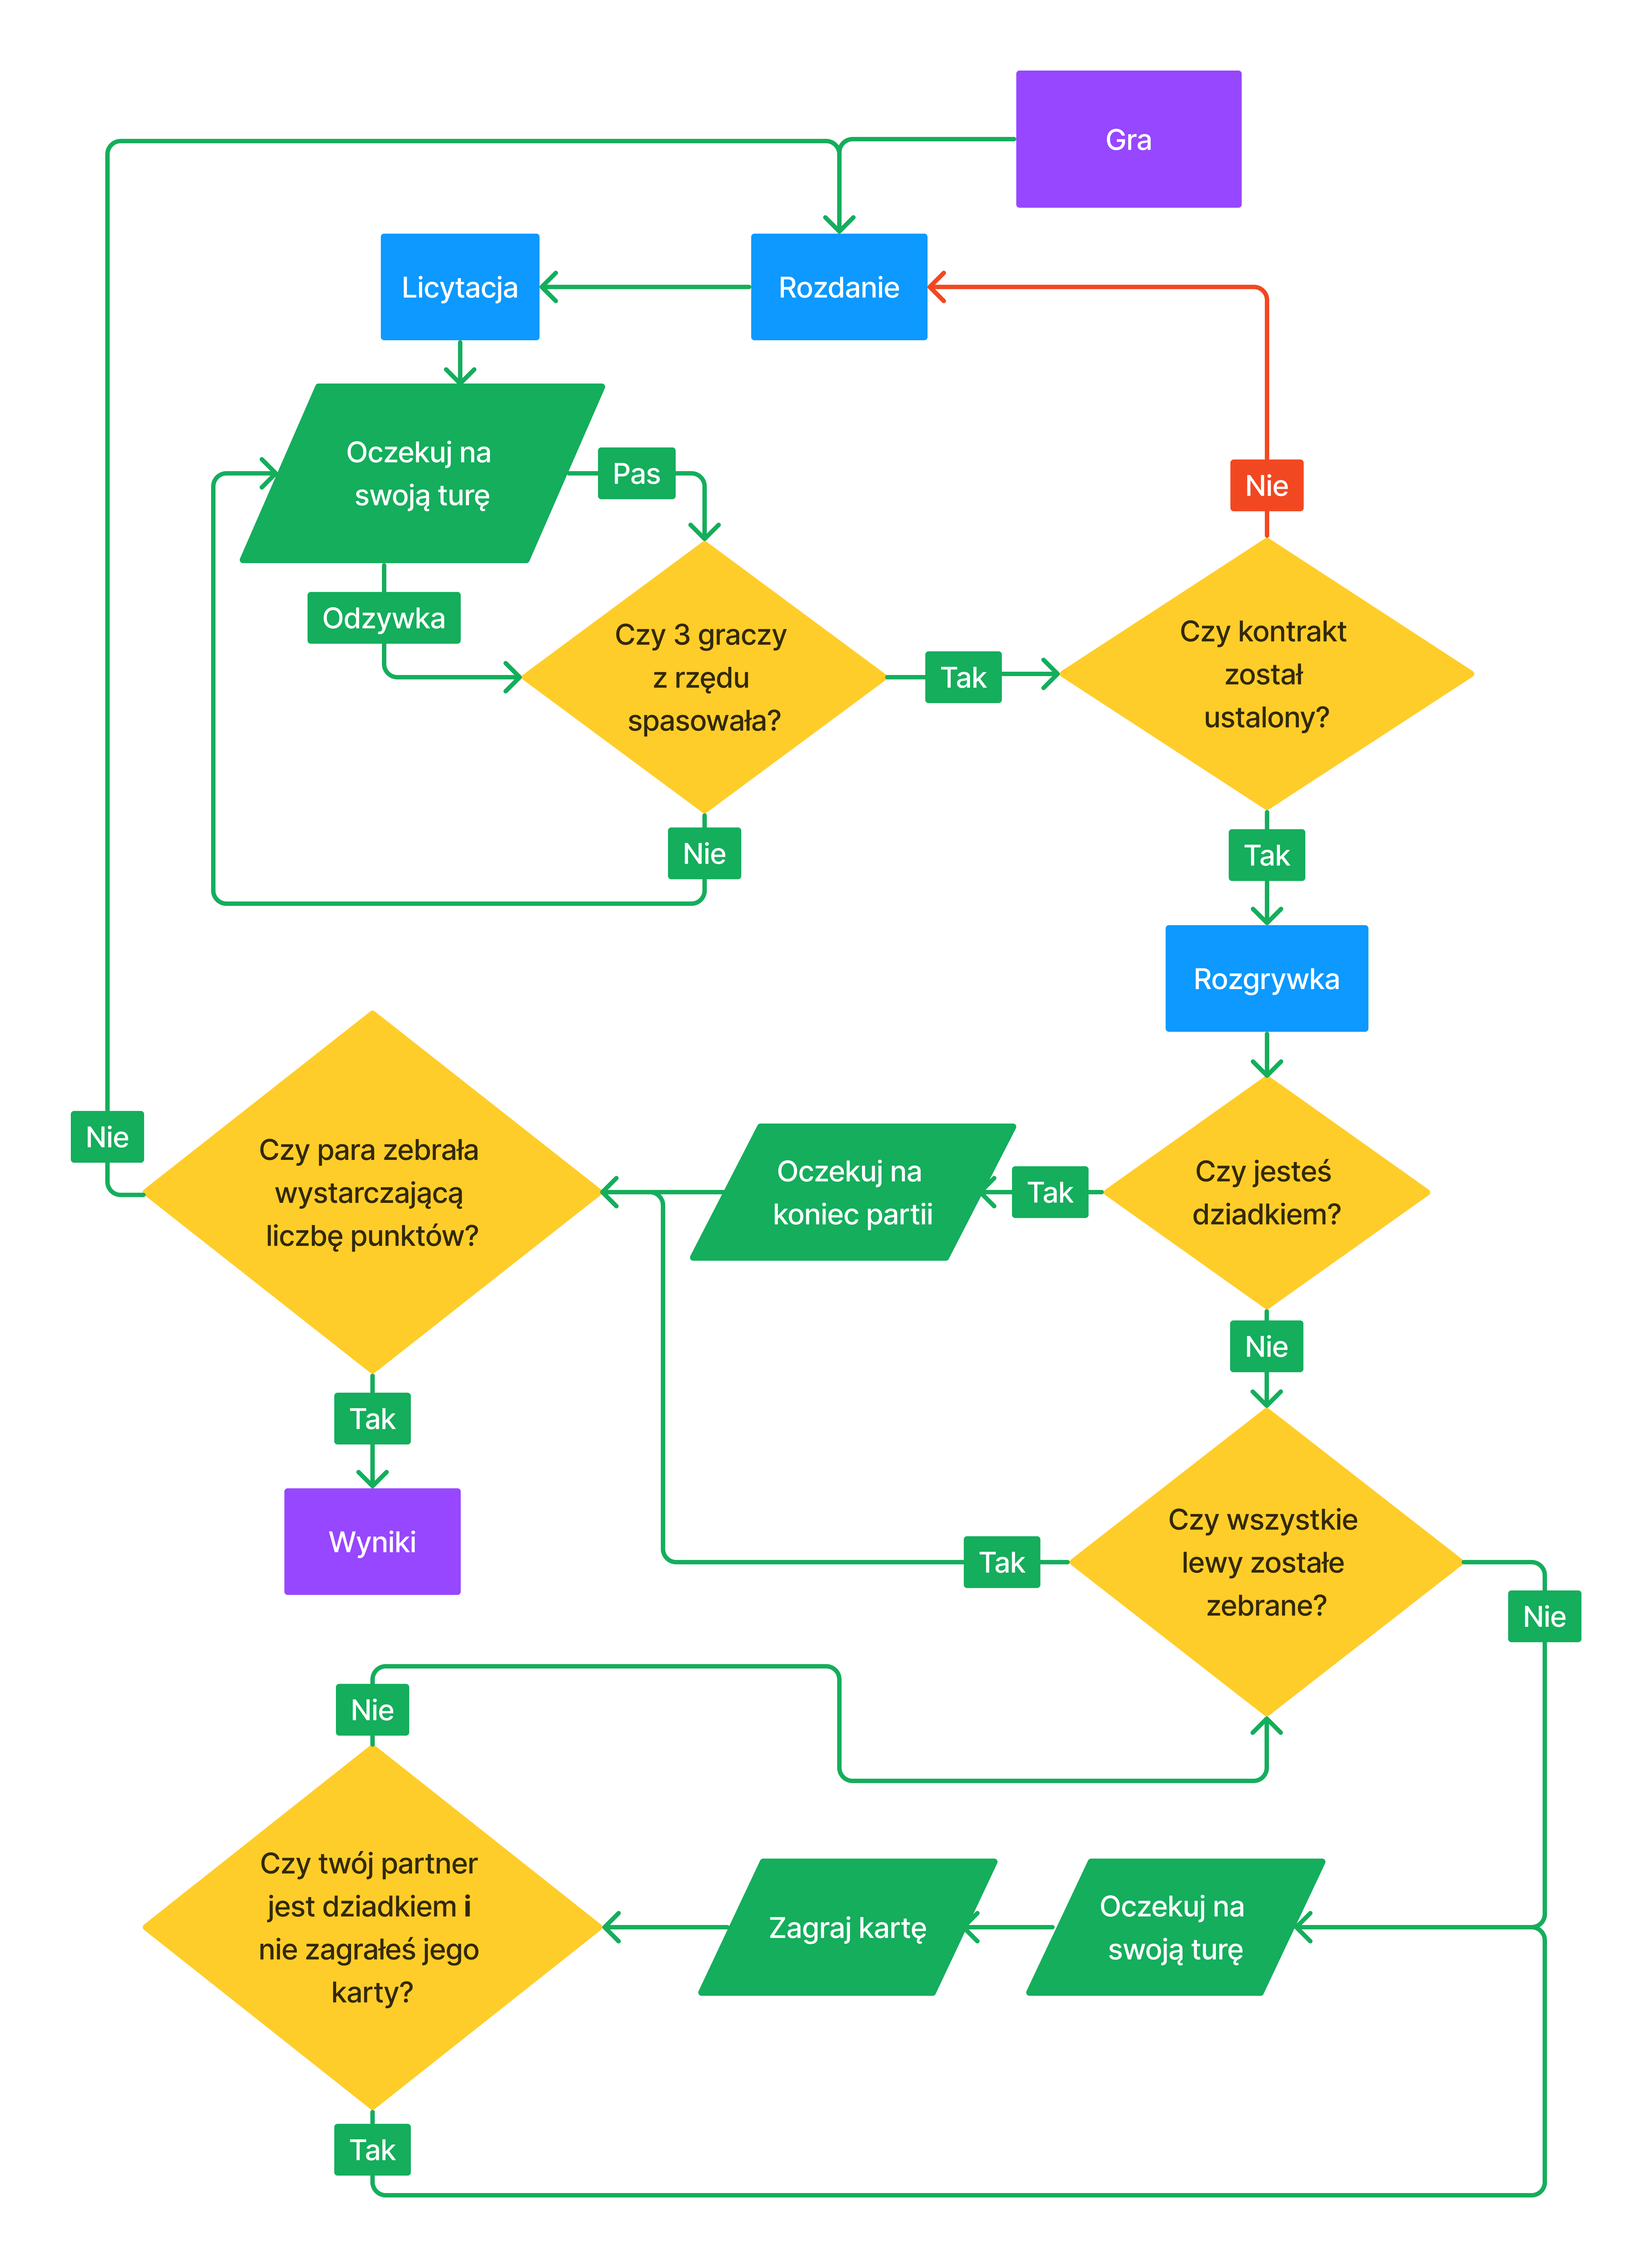
\includegraphics[width=\textwidth]{img/flow-aplikacji/game_flow.png}
  \caption{Schemat interakcji użytkownika z aplikacją podczas rozgrywki brydża}
\end{figure}

\FloatBarrier

\section{Przypadki użycia}

\subsection{Rejestracja/Logowanie do aplikacji}

Aby uzyskać dostęp do większości funkcjonalności aplikacji, wymagane
jest posiadanie konta. Anonimowy użytkownik może je utworzyć, klikając
opcję "\textbf{Register}" w~nagłówku strony. Po kliknięciu użytkownik
zostanie przekierowany do formularza rejestracyjnego.
Do utworzenia konta wymagane jest podanie własnego
pseudonimu, adresu e-mail oraz hasła. Aby uzyskać dostęp do utworzonego
konta, należy kliknąć "\textbf{Log in}" w~nagłówku strony, po czym
w~formularzu podać dane wykorzystanie podczas rejestracji.

W~przypadku nieprawidłowo podanych danych podczas rejestracji
lub logowania, błędów wynikających z~połączeniem internetowym lub
niedostępnym serwerem autentykacji użytkownik otrzyma odpowiednią
informację na ekranie.

\begin{figure}[h]
  \centering
  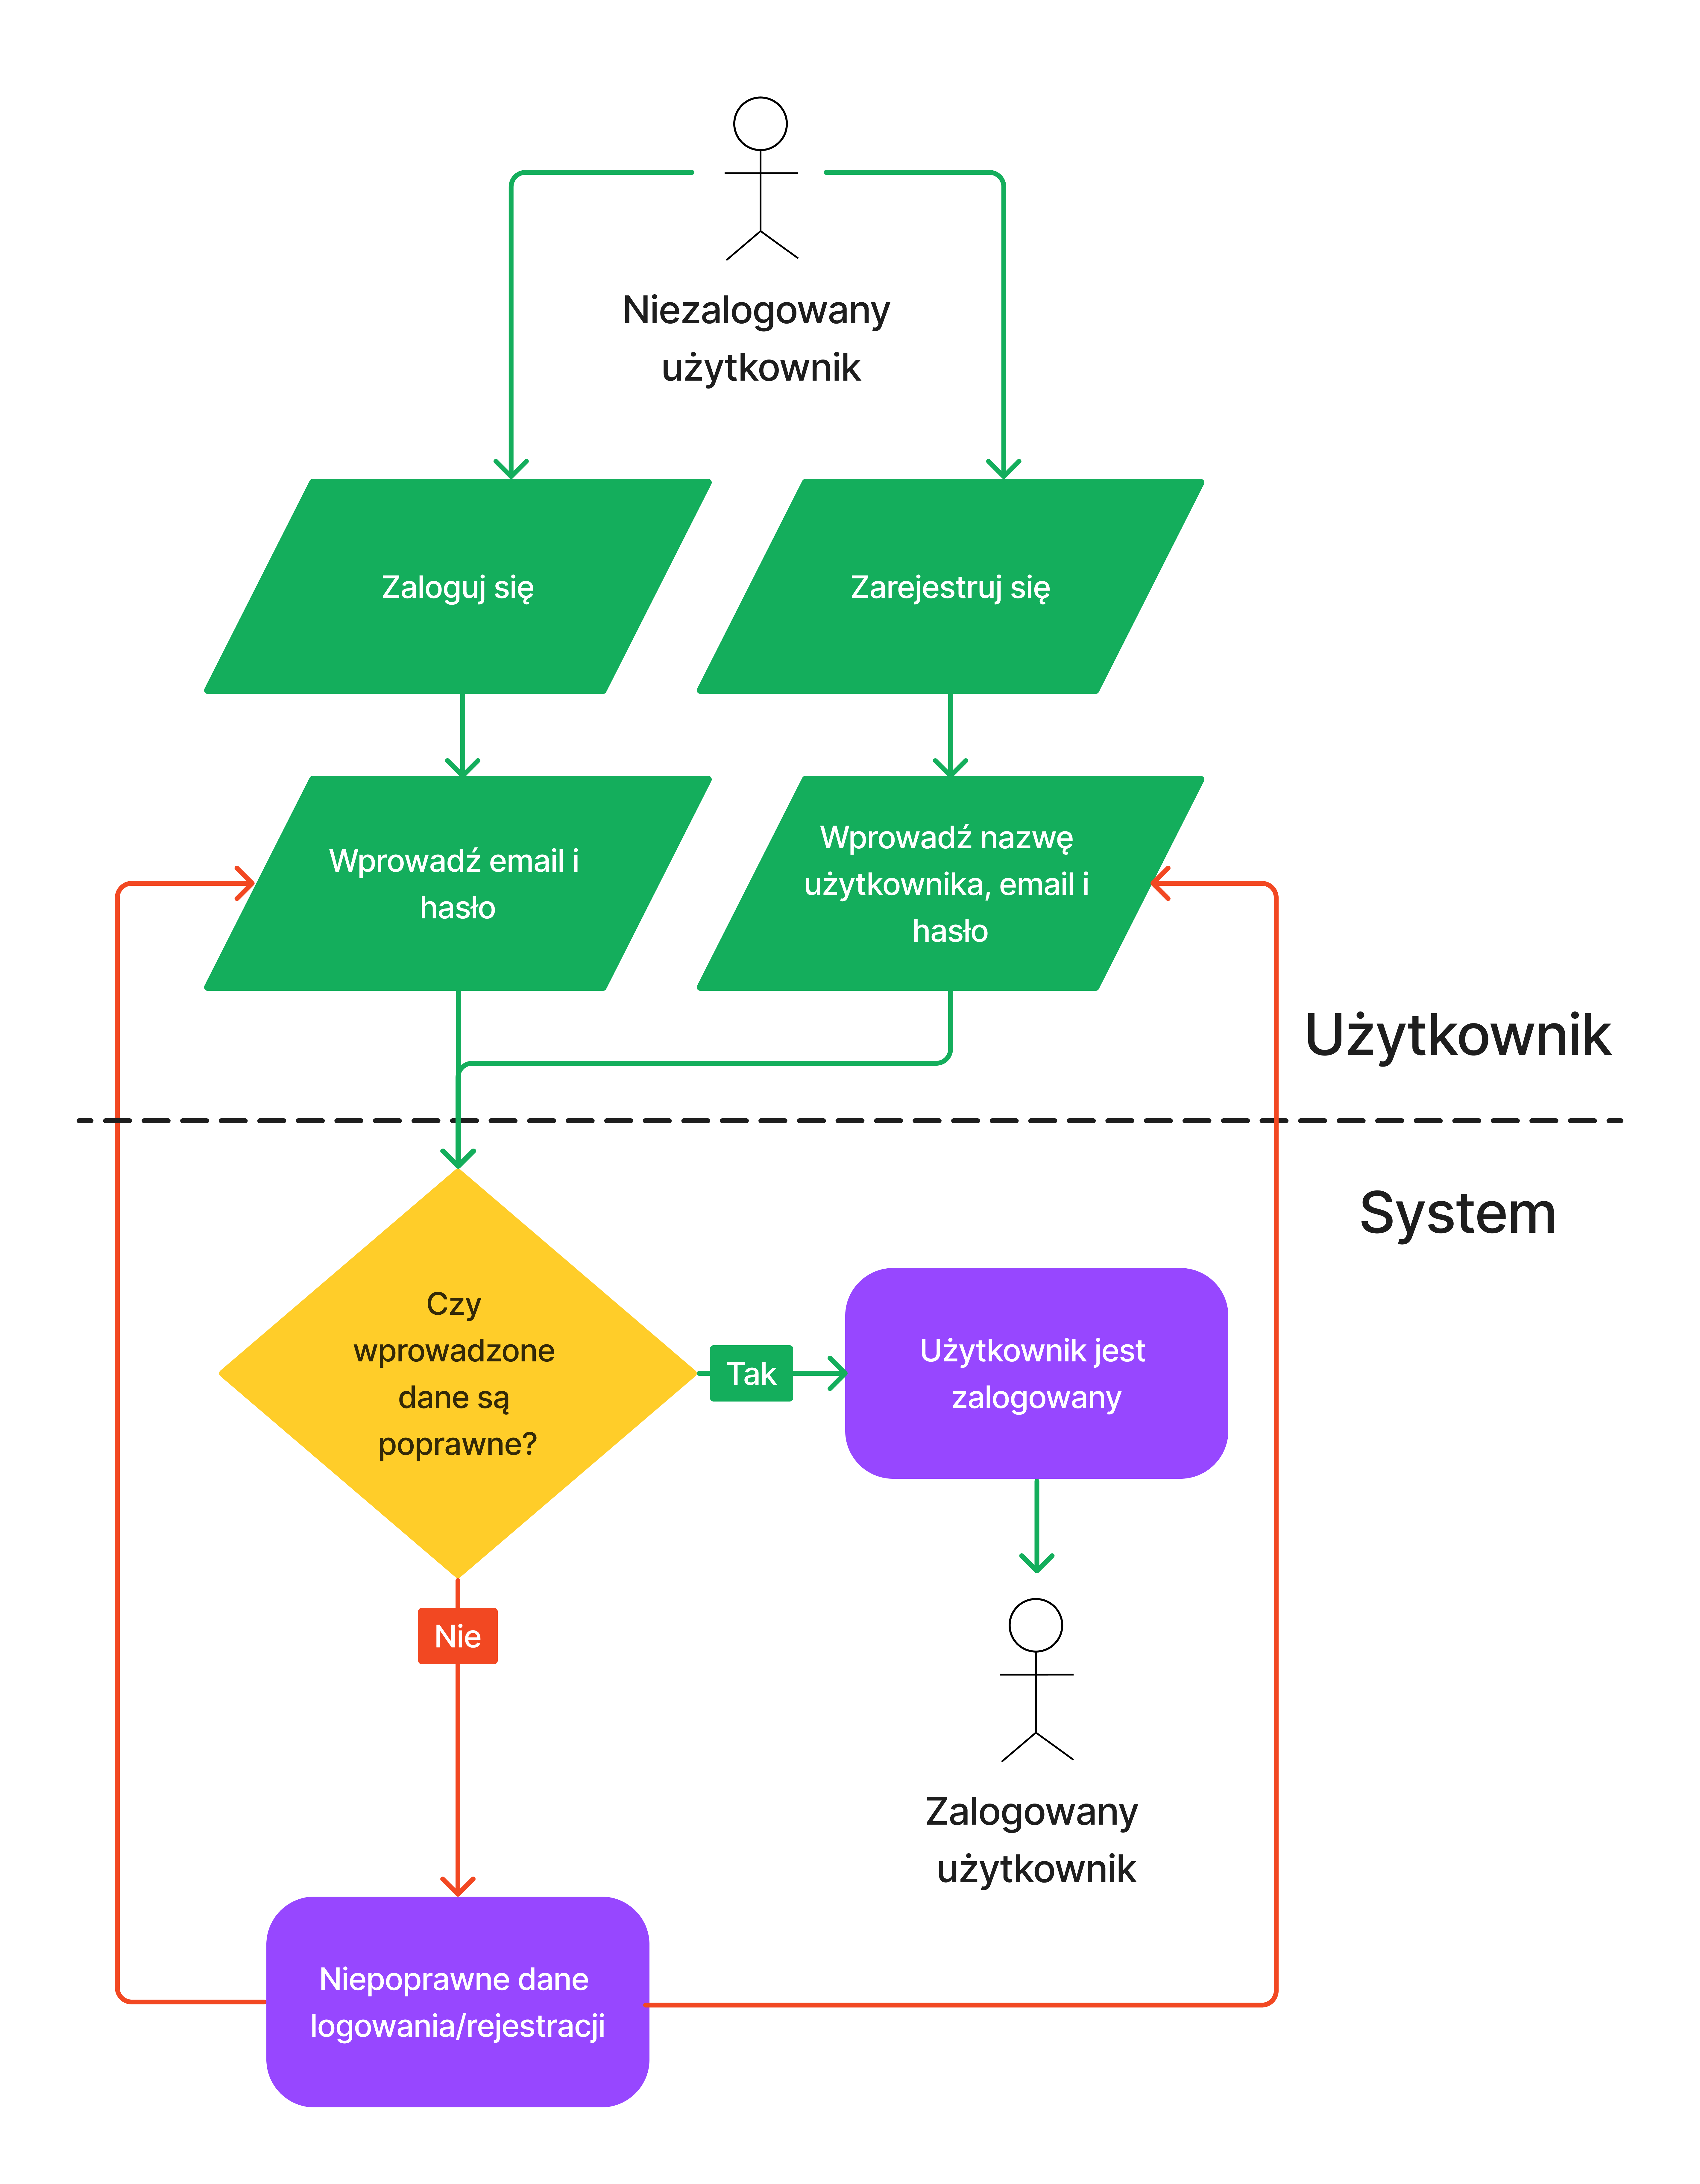
\includegraphics[width=\textwidth]{img/schematy/login.png}
  \caption{}
\end{figure}

\FloatBarrier

\subsection{Tworzenie lobby}

Rozpoczęcie gry w~brydża jest dostępne z~poziomu lobby. Aby utworzyć
lobby, należy kliknąć "\textbf{Create lobby}" na głównym panelu
aplikacji. Przekieruje ono użytkownika do nowego lobby
z~unikalnie wygenerowanym identyfikatorem, którego staje
się administratorem. Użytkownik może udostępnić link do adresu strony,
na której się znajduje, aby udostępnić, np. znajomym swoje lobby, do
którego mogą dołączyć.


\begin{figure}[h]
  \centering
  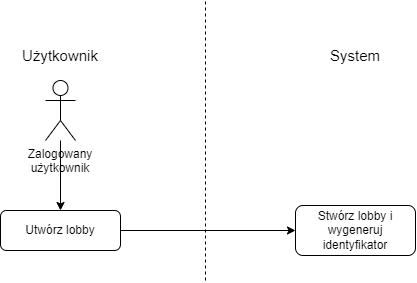
\includegraphics[width=\textwidth]{img/schematy/create_lobby.png}
  \caption{}
\end{figure}

\FloatBarrier

\subsection{Dołączanie do lobby}

Gdy użytkownik otrzyma link do lobby od innego użytkownika, może się
do niego dołączyć, wykorzystując adres strony lobby lub wklejając
identyfikator lobby w~odpowiednie pole w~głównym panelu aplikacji
i~klikając opcję "\textbf{Join}". W~obu przypadkach użytkownik zostanie
przekierowany do lobby.

\begin{figure}[h]
  \centering
  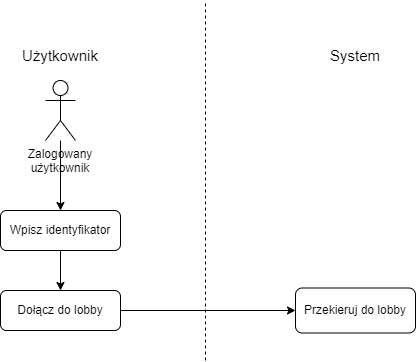
\includegraphics[width=0.7\textwidth]{img/schematy/join_lobby.png}
  \caption{}
\end{figure}

\FloatBarrier

\subsection{Zarządzanie lobby}

Jeżeli użytkownik jest administratorem lub został jedynym
graczem niekontrolowanym przez asystenta AI w~lobby, może on zarządzać graczami znajdującymi się
wewnątrz. Posiada on następujące możliwości:
\begin{itemize}
  \item usunięcie gracza z lobby -- gracz opuszcza lobby i~nie będzie
        mógł już ponownie do niego dołączyć,
  \item przyznanie pozycji w lobby jako AI -- wybrana pozycja
        gracza w~brydżu będzie kontrolowana przez asystenta AI
        i~uczestniczyć w~rozgrywce jako partner lub przeciwnik,
  \item zamknięcie lobby -- jeżeli administrator jest ostatnim ludzkim
        graczem w~lobby, opuszczenie go spowoduje jego automatyczne
        zamknięcie.
        %  \item zmiana statusu lobby na publiczne/prywatne -- powoduje
        %         dostępność rozgrywki rozpoczętej przez lobby w~panelu

\end{itemize}

\begin{figure}[h]
  \centering
  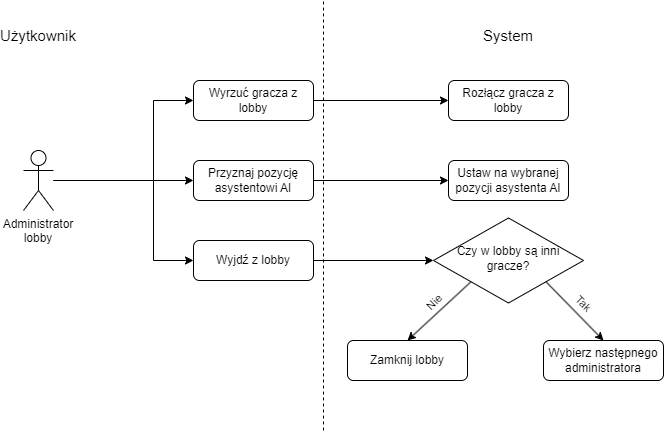
\includegraphics[width=\textwidth]{img/schematy/manage_lobby.png}
  \caption{}
\end{figure}

\FloatBarrier

% \subsection{Obserwowanie rozgrywek}

% Gdy jakaś rozgrywka w~brydża została rozpoczęta i~ma ona status
% publiczny, jest możliwe obejrzenie jej z~panelu \textbf{Watch}.
% Z~listy publicznych rozgrywek należy wybrać interesującą i~kliknąć
% ikonę oka. 
% \end{itemize}

% \begin{figure}[h]
%   \centering
%   \includegraphics[width=\textwidth]{example-image-a}
%   \caption{}
% \end{figure}

% \FloatBarrier


\section{Specyfikacja wymagań funkcjonalnych}
Aplikacja nie tylko powinna być dobrze zaprojektowana i~wygodna
w~użyciu, ale także funkcjonalna. Musi spełniać założone wymagania,
udostępniając odpowiednie funkcjonalności, żeby była przydatna dla
jej użytkowników. Nie da się używać wirtualnego asystenta do gry
w~brydża, jeśli brakuje w nim asystenta AI, czy w~ogóle elementu
rozgrywki. Bez spełnienia kluczowych wymagań funkcjonalnych,
aplikacja praktycznie nie istnieje. W~tym podrozdziale przedstawiamy
te wymagania.
\subsection{Logowanie i rejestracja nowych użytkowników}
Żeby uzyskać dostęp do funkcjonalności naszej aplikacji, potrzebne
jest posiadanie konta i bycie zalogowanym. Z~tego względu koniecznością
jest umożliwienie użytkownikom utworzenia konta, logowania się na
nie i~możliwość późniejszego wylogowania. Formularz rejestracji wymaga
podania adresu e-mail, nazwy użytkownika i~hasła. Logowanie odbywa się
poprzez wprowadzenie swojego adresu e-mail i~hasła.
\subsection{Utworzenie/Dołączenie do lobby}
W celu rozegrania partii brydża przeciwko innym graczom bądź
przeciwnikom AI, gracz musi mieć możliwość utworzenia własnej
rozgrywki oraz dołączenia do istniejącej. Utworzenie, jak i~dołączenie do
lobby jest dostępne z~widoku głównego aplikacji. Dołączenie do lobby
odbywa się poprzez wprowadzenie identyfikatora gry lub wejście w~link
otrzymany od założyciela lobby. Po utworzeniu lobby użytkownik może
wysłać jego identyfikator innym graczom, zapraszając ich do dołączenia,
albo zdecydować się na wypełnienie brakujących miejsc asystentami AI.
\subsection{Wyrzucenie gracza z lobby}
Administrator lobby może w dowolnym momencie arbitralnie wyrzucić
każdego z pozostałych graczy.
\subsection{Rozpoczęcie rozgrywki}
Kiedy do lobby dołączą wszyscy gracze lub część miejsc zostanie
obsadzonych asystentami AI, administrator lobby może rozpocząć
rozgrywkę, używając odpowiedniego przycisku. Wszyscy gracze zostają
przeniesieni do ekranu gry.
\subsection{Rozgrywka}
Głównym celem i~podstawową funkcjonalnością naszej aplikacji jest
rozgrywka w brydża. Każda runda zaczyna się od licytacji, po której
gracze wykładają karty zgodnie z~zasadami gry. Gra kończy się, kiedy
jedna z~par zdobędzie wystarczającą liczbę punktów. Po skończonej
rozgrywce użytkownikowi wyświetlany jest ekran z~wynikami.
\subsection{Wyświetlenie wyników}
Ważne jest, żeby gracze po skończeniu partii mogli zobaczyć
podsumowanie całej rozgrywki. Użytkownikowi wyświetlany jest ostateczny
wynik gry, a~także liczba zdobytych punktów przez jego zespół na
podstawie zdobytych lew. Dzięki temu gracze mogą dokładniej
przeanalizować rozegraną partię i~lepiej oceniać swoje możliwości
podczas licytacji w~przyszłych rozgrywkach.
\subsection{Opuszczenie rozgrywki}
Użytkownik może nie tylko wyjść z~lobby, ale także w~dowolnym momencie
opuścić rozgrywkę. W~takim przypadku miejsce gracza zastępuje
asystent AI.
% TODO

\section{Specyfikacja wymagań niefunkcjonalnych}
W naszym projekcie aplikacji -- wirtualnego asystenta do gry w~brydża,
istotą jest zapewnienie nie tylko wszystkich potrzebnych wymagań
funkcjonalnych, ale także wygodnej i~przyjemnej rozgrywki oraz
korzystania z reszty funkcjonalności. Niewiele osób będzie chętnie
korzystać z~aplikacji, choćby miała ona wyjątkowo rozbudowane spektrum
funkcji, jeśli jej działanie będzie niestabilne i~pozbawione
intuicyjności. W~tym podrozdziale przedstawiamy wymagania
niefunkcjonalne aplikacji, które są równie ważne, jak zdefiniowane
wcześniej wymagania funkcjonalne.
\subsection{Dostępność}
Rozwijany przez nas wirtualny asystent do gry w~brydża jest aplikacją
webową. Dzięki temu będzie on dostępny zarówno dla użytkowników
Windows, MacOS, Linux, jak i~innych systemów operacyjnych posiadających
przeglądarkę wspierającą najnowsze standardy. Co więcej, starannie
zaprojektowane interfejsy użytkownika (UI) zostały dostosowane tak,
aby były wygodne i~funkcjonalne nawet na urządzeniach o~niewielkich
rozmiarach ekranu, umożliwiając płynne korzystanie z~aplikacji również
na urządzeniach mobilnych.
\subsection{Użyteczność}
Priorytetem naszej aplikacji jest zapewnienie łatwości obsługi
i~zrozumiałości. Niezwykle istotne jest, aby interfejs użytkownika
był intuicyjny, estetyczny i~nie zniechęcał potencjalnych użytkowników,
ani nie utrudniał korzystania z~aplikacji. Dlatego podczas projektowania
interfejsu użytkownika kierowaliśmy się zasadami dobrego UI/UX.
Stworzyliśmy minimalistyczny i~uporządkowany interfejs, który eliminuje
chaos i~zapewnia spójność na wszystkich podstronach aplikacji.
Wykorzystaliśmy ikony o~jednakowym znaczeniu na wszystkich stronach,
co ułatwia nawigację. Dodatkowo zastosowaliśmy stałą gamę starannie
dobranych kolorów dla elementów interfejsu, co pozwoliło nam utrzymać
spójny styl podczas projektowania kolejnych widoków. Aplikacja oferuje
tryb jasny i~ciemny, aby użytkownicy mogli wygodnie korzystać z~niej
w~zależności od preferencji lub pory dnia. Ponadto, wszystkie podstrony
są responsywne, co oznacza, że elementy interfejsu zachowują pełną
funkcjonalność, niezależnie od zmiany rozmiaru ekranu, na którym są
wyświetlane.
\subsection{Niezawodność}
Wirtualny asystent do gry w brydża tworzony jest z~myślą o~nauce
i~doskonaleniu umiejętności, ale także konkurencji i~wzajemnym
rozgrywkom pomiędzy graczami. Konieczne jest więc wprowadzenie logiki
gry z~największą dokładnością. Błędy w działaniu aplikacji podczas
rozgrywki mogłyby wpłynąć na wynik gry oraz wprowadzić nowych graczy
w~zakłopotanie, a~bardziej doświadczonych w~stan irytacji.
Niezwykle istotne jest również uniknięcie sytuacji, w~których
dochodziłoby do utraty połączenia lub braku synchronizacji pomiędzy
graczami. Takie incydenty mogą zrujnować całą rozgrywkę i~zdecydowanie
obniżyć wartość jednej z~kluczowych funkcjonalności aplikacji, jaką
jest możliwość rozgrywania partii między użytkownikami.
Pierwszym krokiem w~stronę niezawodności aplikacji było wybranie
odpowiednich technologii do jej realizacji. Next.js oraz FastAPI %%% TODO dowód?
to godne zaufania, popularne na całym świecie narzędzia do budowy
aplikacji webowych, a~usługa Google Firebase odciąża nas z~implementacji
funkcjonalności gromadzenia danych i~obsługi użytkowników od podstaw.
Mając odpowiedni stos technologiczny, przystąpiliśmy do implementacji
kolejnych funkcjonalności z~najwyższą starannością.



\chapter{\ChapterTitleRealizationAspects}
\label{sec:wybrane-aspekty-realizacji}

Ta sekcja pracy skupia się na najważniejszych aspektach opracowanej
aplikacji, podkreślając istotne modyfikacje przeprowadzone w~trakcie
jej implementacji. Jej celem jest szczegółowe opisanie poszczególnych
komponentów oraz zidentyfikowanie czynników, które mogły prowadzić do
ewentualnych błędów w~funkcjonowaniu systemu. Dodatkowo skoncentruje
się na prezentacji skutecznych rozwiązań dla wykrytych problemów,
oferując konkretne przykłady, które ilustrują zastosowane poprawki.

\section{Architektura serwera}

%%% TODO expand basic info
Serwer napisany w języku Scala.

\subsection{Połączenia z serwerem}

Wstępne założenia dotyczące infrastruktury aplikacji
serwerowej opierały się na wykorzystaniu języka Python
wraz z~frameworkiem FastAPI. Z~czasem jednak, w~świetle
narastających wymagań i~doświadczeń zgromadzonych
podczas etapu tworzenia, nasz zespół podjął
strategiczną decyzję o~ewolucji stosu technologicznego.
Ostatecznie, struktura serwera została skonstruowana
w~dynamicznym języku Scala, korzystając z~potencjału
frameworku Akka, specjalizującego się w~programowaniu
współbieżnym oraz rozproszonym, bazującym na
zaawansowanym modelu aktorów.

Pierwotny model komunikacji między klientem, a~serwerem
był zbudowany w~oparciu o~metodę \textbf{short polling},
%%% TODO jakiś słownik co znaczy short polling???
zaimplementowaną przy pomocy FastAPI. Ten sposób
w~praktycznym zastosowaniu ujawnił pewne ograniczenia.
Regularne zapytania wysyłane przez klienta w~celu
sprawdzenia stanu danych na serwerze prowadziły do
znacznych opóźnień w~aktualizacji interfejsu
użytkownika. Taka sytuacja stwarzała trudności nawet
przy realizacji bardzo prostych funkcji, takich jak
zmiana pozycji użytkowników w~przestrzeni lobby.

Wobec wyzwań, narzuconych przez ograniczenia wyżej wspomnianej metody, nasz
zespół rozważał migrację ku strategii \textbf{long polling}. Metoda ta,
w~odróżnieniu od konwencjonalnych technik polegających na ciągłym
wysyłaniu zapytań przez klienta w~celu odświeżenia danych, proponuje
utrzymanie otwartego kanału HTTP do czasu, aż serwer będzie miał
najnowsze informacje do przekazania. Mimo iż koncepcja ta wydawała się
obiecująca, powstały obawy związane z~koniecznością ciągłego monitorowania
potencjalnej utraty połączenia. Skłoniło nas do ostatecznej rezygnacji
z~wdrożenia tego pomysłu.

Implementacja frameworku Akka pozwoliła na ustanowienie stabilnego,
\textbf{reaktywnego} połączenia między klientem a~serwerem. Programowanie
reaktywne, koncentrujące się na płynnym przepływie danych i~ich propagacji,
umożliwiło aplikacji klienta natychmiastowo reagować na wszelkie zmiany. Jest
to szczególnie istotne w~kontekście naszej aplikacji, która charakteryzuje
się intensywną interakcją użytkownika, zwłaszcza podczas naszej kluczowej
funkcjonalności -- rozgrywki w~brydża. Zastosowanie tego podejścia
znacząco usprawniło koordynację sekwencji animacji ruchów poszczególnych
graczy.

%%% mozna opisac to pozniej
% \subsection{Testy}
% Framework Akka dostarcza także kompleksowe narzędzia do efektywnego
% testowania aktorów, w~tym symulowane środowisko czasu wykonania, które
% pozwala na dogłębne sprawdzenie zachowań asynchronicznych w~warunkach
% synchronicznych. Dzięki tym możliwościom możemy rozwijać architekturę
% serwera, mając pełne przekonanie co do jej stabilności i~niezawodności
% działania.

\section{Aplikacja webowa}
Aplikacja webowa została stworzona przy użyciu platformy Next.js oraz
języka programowania Typescript, będącego rozszerzeniem Javascriptu
o~statyczne typowanie. Ta część projektu została zrealizowana zgodnie
z~pierwotnymi założeniami. Jednakże wyjątkiem było wdrożenie funkcji
rozgrywki w~brydża. Ze względu na złożoność problemów i~wymagania
dotyczące wydajności, zdecydowano się na implementację tego elementu za
pomocą technologii wcześniej niewzględnie planowanej.

Warto zaznaczyć, że implementacja rozgrywki w~brydża została logicznie
odseparowana od reszty aplikacji, choć w~pełni integruje się z~samą
platformą i~korzysta z~wcześniej wspomnianych języków programowania.
Szczegółowy opis części znajduje się w~podrozdziale \nameref{subsec:silnik_gry}.


\subsection{Przystosowanie do backendu -- hooki}
Biblioteka React oferuje potężne narzędzie w postaci hooków, które umożliwiają efektywne zarządzanie stanem i cyklem życia komponentów. W naszym projekcie, do obsługi zapytań klienta do serwera backendowego, zdecydowaliśmy się skorzystać z hooka useSWR, pochodzącego z biblioteki SWR. Jest to wysoce efektywne rozwiązanie do pobierania danych w aplikacjach opartych na React. Aby jeszcze bardziej zoptymalizować proces, stworzyliśmy również zestaw własnych, dedykowanych hooków. Takie podejście pozwoliło na znaczną standaryzację logiki odpowiedzialnej za wysyłanie i odbieranie zapytań HTTP, co przyczyniło się do drastycznego zmniejszenia ilości kodu wymaganego do realizacji tych operacji.
\subsection{Efektywne opisywanie stylu}
W celu nadania stylów komponentom naszej aplikacji internetowej posłużyliśmy się frameworkiem Tailwind CSS w połączeniu z biblioteką Daisy UI. Zastosowanie gotowych klas dostarczonych przez te narzędzia umożliwiło nam efektywne i intuicyjne stylizowanie elementów interfejsu użytkownika, eliminując jednocześnie potrzebę bezpośredniego zarządzania plikami CSS. Dzięki temu uniknęliśmy konieczności definicji własnych klas, co często prowadzi do tworzenia zawiłego i powtarzalnego kodu. Wykorzystanie tego podejścia znacznie przyspieszyło proces rozwoju front-endu naszej aplikacji.
\subsection{Testy E2E}


\section{Silnik gry}
\label{subsec:silnik_gry}
Próba implementacji animacji, takich jak ruch kart, z wykorzystaniem wyłącznie komponentów React okazała się być nadmiernie czaso i pracochłonna. Ta część projektu została dokładniej omówiona w sekcji poświęconej Silnikowi gry.

\subsection{Integracja silnika z React'em}


\section{AI}

\subsection{TBC}


\chapter{\ChapterTitleWorkOrganization}
\label{sec:organizacja-pracy}

\section{Historia pomysłu projektu}

%%% jak było

\section{Charakterystyka i sposób realizacji projektu}

%%% bardzo ogólna wizja co chcemy mieć
%%% jak podzieliliśmy głowne częsci całej aplikacji
%%% core, backend, front, game-engine, thesis

\section{Weryfikacja postępów w trakcie realizacji}

\subsection{Milestone'y}
%%% najpierw base, pozniej lobby, pozniej gra a na koncu gra z ai
%%% scisle powiazane z epicami

\subsection{Spotkania z promotorem}
%%% to opisujmey w obu przypadkach \subsubsection{Microsoft Teams}

\subsection{Pracownia projektowa}
%%% to opisujmey w obu przypadkach \subsubsection{Microsoft Teams}


\section{Zastosowane praktyki i narzędzia organizacji pracy}

\subsection{Planowanie i projektowanie}

\subsubsection{Shortcut}

\subsubsection{Figma}


\section{Wykorzystywane technologie do realizacji projektu}

\subsection{Komunikacja wewnętrzna}

W trakcie tworzenia projektu potrzebna była szybka i efektywna
wymiana wiadomości oraz możliwość współpracy w czasie rzeczywistym.
Wykorzystana została w tym celu platforma Discord~\cite{Discord},
która oferuje rozmowy głosowe, kanały tekstowe i udostępnianie
obrazu na żywo.


\subsection{System kontroli wersji}

Aby synchronizować postępy pracy i ich historię zastosowano
system kontroli wersji Git \cite{Git}. Wraz z nim, do przechowywania
repozytoriów z kodem aplikacji, jak i dokumentacji wykorzystano
platformę GitHub \cite{Github}.

\subsection{Tworzenie dokumentacji}

Do napisania dokumentacji aplikacji użyto języka \LaTeX~\cite{Latex}.
Przesyłając tekst pracy na platformę GitHub, skorzystano z~technologii
GitHub Actions \cite{GithubActions}, którą wykorzystano w celu
generacji dokumentu od razu po opublikowaniu zmian w~tekście pracy.
Umożliwiło to na dostęp do najnowszej wersji dokumentu dla opiekuna
pracy i~prowadzącego pracownię projektową, dzięki czemu była możliwa
ciągła weryfikacja postępów nad pracą.


\subsection{Tworzenie oprogramowania}

\subsubsection{VSCode}

\subsubsection{Produkty Jetbrains}

\subsubsection{Postman}


\subsection{Wdrażanie i testowanie}

\subsubsection{Github Actions (deploy \& tests)}

%%%\subsubsubsection{Konteneryzacja (repozytorium)}

\subsubsection{Oracle Cloud (backend)}

\subsubsection{Vercel (front)}


\chapter{\ChapterTitleResults}
\label{sec:wyniki-projektu}

\section{Weryfikacja realizacji wstępnych założeń}
%%% bardzo ogolne
%%% czy udało nam sie zrealizowac projekt i wszystkie zalozenia
%%% z wczesniejszych rozdzialow

%%% opisac funkcje produktu czy zostaly zrealizowane/w jaki sposob
\subsection{funkcja1}
\subsection{funkcja2}
\subsection{funkcja3}

\subsection{Porównanie pokrycia z planem interfejsu}
% porownanie z figmą jaki powstal system (u nas udal sie caly)


\section{Przegląd zrealizowanych funkcjonalności}

\subsection{Interfejs aplikacji}

\subsubsection{Tworzenie i dołączenie do gry}
\subsubsection{Lobby}
\subsubsection{Host}
\subsubsection{Użytkownik}


\subsection{Gra w brydża}

\subsubsection{Licytacja}
\subsubsection{Rozgrywka}


\subsection{Wirtualny asystent}
%%% przeprowadzone testy aplikacji na wybranej grupie osób

\subsubsection{Moc AI}
%%% testy/badania czy AI wygrywa


\subsection{Ułatwienia dostępności}

Oprócz omówionych kluczowych funkcjonalności, w~ramach rozwoju
aplikacji wprowadzono także dodatkowe elementy, których
potrzebę przedstawiono w~podrozdziale dotyczącym wymagań
niefunkcjonalnych. Głównych ich celem było zapewnienie
wygody i~prostego korzystania z~aplikacji, nawet podczas
pierwszego użytkowania. Poniżej przedstawione rozwiązania powstały
z~inicjatywy zespołu. Zostały one zaakceptowane przez klienta,
realizując wymagania dostępności i~użyteczności.

\subsubsection{Intuicyjność interfejsu}

Aby aplikacja była intuicyjna dla każdego użytkownika,
zastosowano ikony wprost kojarzące się z~wykonywaną
przez nie akcją. Zastosowano wyróżniające się kolory wśród palety
aplikacji w~celu podkreślenia danych czynności wykonywanych
przez użytkownika (Rys. \ref{fig:host_actions_ui}). Kontrastowe barwy mają zwrócić uwagę na
skutki danej akcji. Przykładowo jaskrawy czerwony kolor
kojarzący się przemocą lub impulsywnością wraz z~ikoną
przedstawiającą "$\times$"\xspace odpowiada za wyrzucenie gracza
z~sesji. Zastosowanie wspomnianych technik przestrzega
użytkownika przed przedwczesnym kliknięciem, ale także kojarzą
się one z~negatywną czynnością.

\begin{figure}[h!]
  \centering
  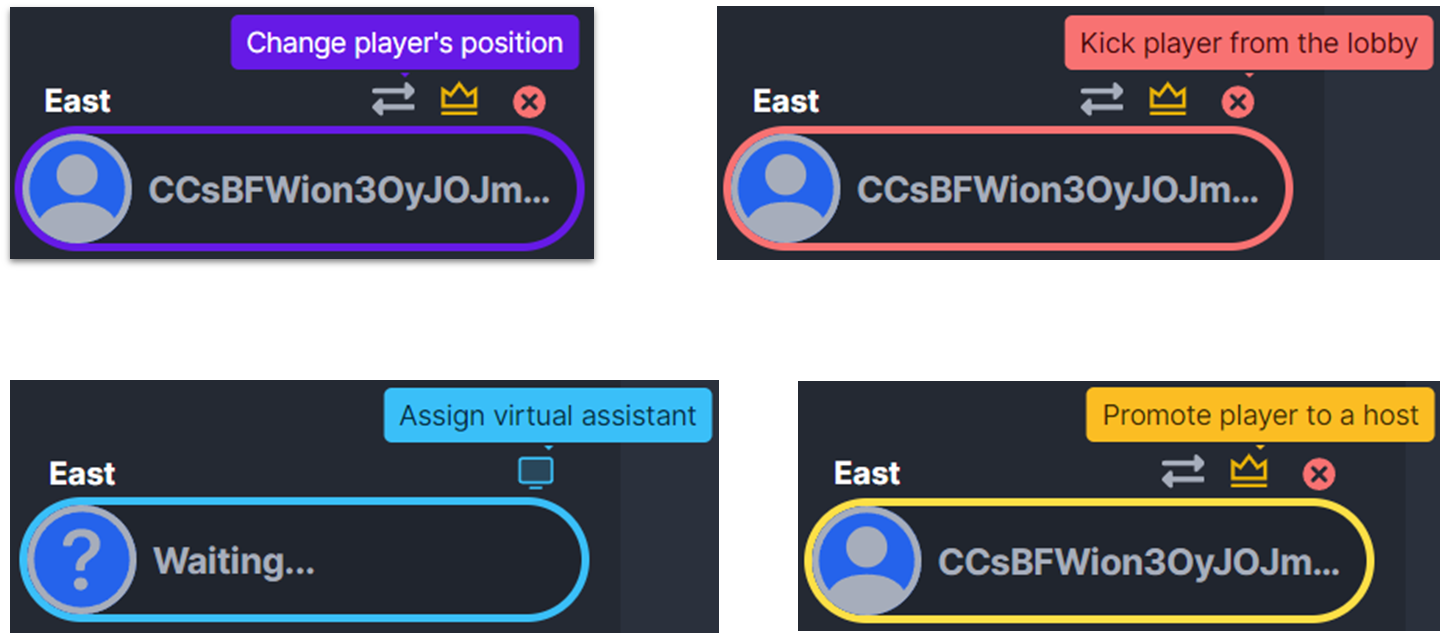
\includegraphics[width=\textwidth]{img/widoki/host_actions.png}
  \caption{Akcje hosta lobby}
  \label{fig:host_actions_ui}
\end{figure}

\FloatBarrier

\subsubsection{Responsywny układ aplikacji}

Zgodnie z~wymogiem dostępności interfejsy aplikacji powinny
być funkcjonalne również na urządzeniach o~niewielkich
rozmiarach ekranu. Wszystkie strony zostały zaprojektowane
tak, aby umożliwić wygodne korzystanie zarówno na urządzeniach
stacjonarnych, jak i~mobilnych (Rys. \ref{fig:responsive_ui}). Aplikacja dynamicznie
dostosowuje się w~zależności od aktualnego rozmiaru okna
przeglądarki.

Minimalna przewidziana
szerokość ekranu wynosi 280 pikseli, dzięki czemu wspierane
są także starsze urządzenia o~niewielkiej rozdzielczości
ekranu.

\begin{figure}[h!]
  \centering
  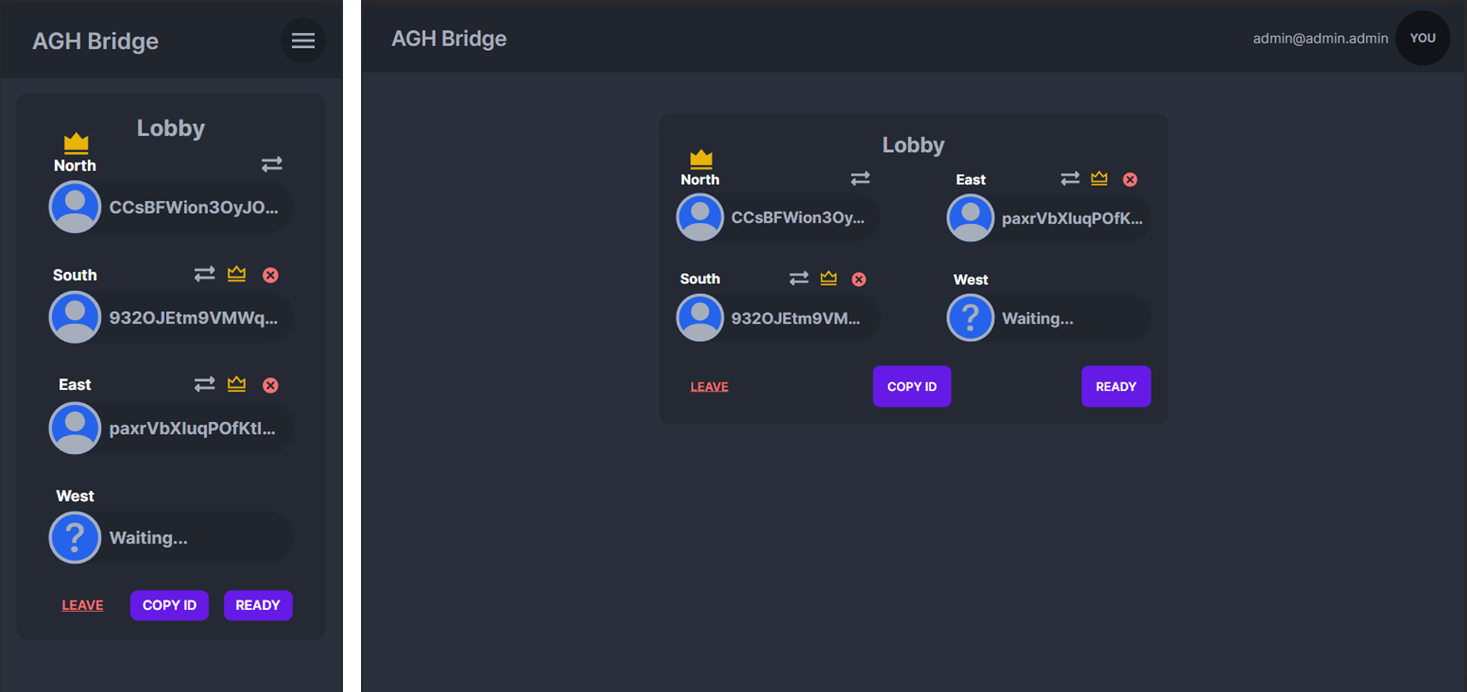
\includegraphics[width=\textwidth]{img/widoki/desktop_mobile.png}
  \caption{Tryb mobilny i desktopowy aplikacji}
  \label{fig:responsive_ui}
\end{figure}

\FloatBarrier

\subsubsection{Motywy jasny i ciemny}

Wygląd aplikacji został zrealizowany w~dwóch trybach --
jasnym i~ciemnym (Rys. \ref{fig:themes_ui}). Użyto w~tym celu dostępnych w~bibliotece
palet kolorów, ale także zdefiniowano własne, aby zachować
motyw kolorystyczny aplikacji. W~zależności od aktualnie
wybranego motywu kolory zmieniały swój odcień.

% \begin{figure}[h!]
%   \centering
%   \includegraphics[width=\textwidth, draft=true]{example-image}
%   \caption{Motywy jasny i ciemny aplikacji}
%   \label{fig:themes_ui}
% \end{figure}

% \FloatBarrier

\begin{figure}[h!]
  \centering
  \begin{minipage}[b]{0.45\textwidth}
    \centering
    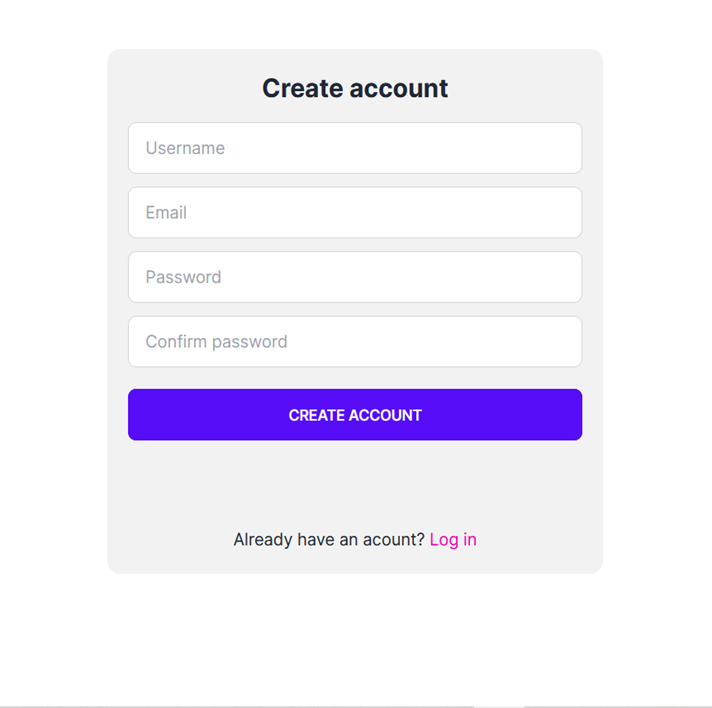
\includegraphics[width=\textwidth]{img/widoki/light.png}
  \end{minipage}%
  \hspace*{0.5cm}
  \begin{minipage}[b]{0.45\textwidth}
    \centering
    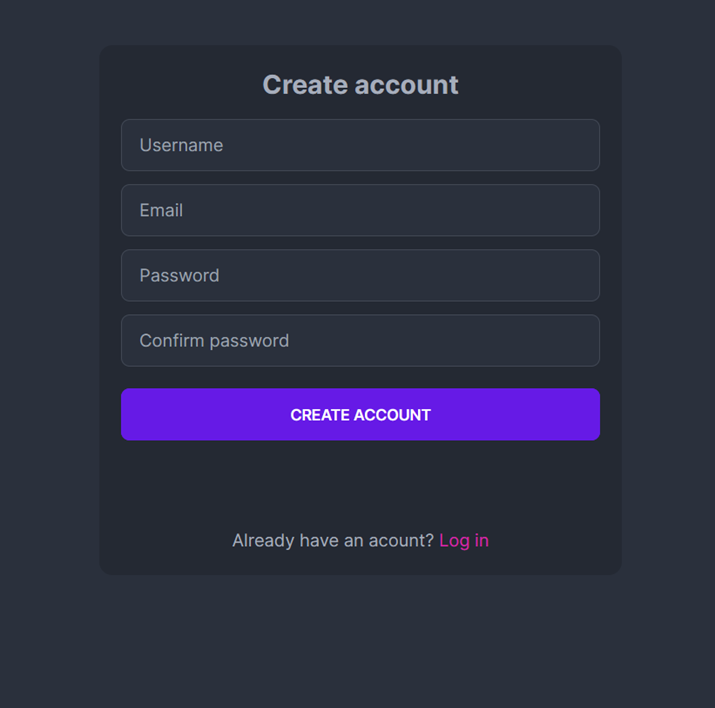
\includegraphics[width=\textwidth]{img/widoki/dark.png}
  \end{minipage}
  \caption{Motywy jasny i ciemny aplikacji}
  \label{fig:themes_ui}
\end{figure}

\FloatBarrier

\section{Dalsze perspektywy rozwoju projektu}

\section{Podsumowanie}




%%%%%%%%%%%%%%%%%%%%%%%%%%%%%%%%%%%%%%%%%%%%%%%%%%%%%%%%%%%%%%%%%%%%%%%%%%%%%%%

\printbibliography

%%%%%%%%%%%%%%%%%%%%%%%%%%%%%%%%%%%%%%%%%%%%%%%%%%%%%%%%%%%%%%%%%%%%%%%%%%%%%%%

\listoffigures
\listoftables
\listofalgorithmes
\lstlistoflistings

\end{document}
